%\documentclass[onecolumn,apj,iop,tighten]{emulateapj2}
\documentclass[apj,tighten,iop]{emulateapj2}

% [Figures] ---------------------------------------------------------------
\usepackage{epstopdf}
%\usepackage[outdir=./figures/]{epstopdf}
%\usepackage[outdir=/figures/]{epstopdf}

% [Bibliography] ---------------------------------------------------------------
\usepackage{natbib}
\citestyle{aa} 
\bibliographystyle{apj} % official 
% \bibliographystyle{apjurl} % with nice links
% \bibliographystyle{tony-apj} % from Alison

% [Colors and the sort] --------------------------------------------------------
\usepackage[usenames]{color}
\definecolor{red}{rgb}{0.75,0,0}
\definecolor{green}{rgb}{0,0.5,0}
\definecolor{blue}{rgb}{0,0,0.75}
\usepackage[ colorlinks=true, % false for boxed links
             urlcolor=blue,
             filecolor=blue,
             linkcolor=red,
             citecolor=blue,
             pdftitle={pdf title},
             pdfauthor={pdf author},
             pagebackref, % Add for citation links
             % pdfpagemode=UseOutlines,
             % backref=page,
             bookmarks,
             bookmarksopen=true]{hyperref}

% [Nice Things] ----------------------------------------------------------------
% \usepackage[sc]{mathpazo} % Better Font. [Looks nice, but not using.]
% \usepackage{lmodern} % Nice PS Text Font. [Not needed]
\usepackage{xspace}    % space after new command
\usepackage{microtype} % Cleans up spacing.
\usepackage{amsmath}  % Some nice math things
\usepackage{amssymb}
\usepackage{float}
\usepackage{booktabs}

% \usepackage[textsize=small,
%             textwidth=0.5in,
%             % disable,
%             backgroundcolor=lightgray]{todonotes} % Fancy ToDo Setup.
% \newcommand{\itodo}[1]{\todo[inline]{#1}}
% \newcommand{\comment}[1]{\todo[inline,
%                                color=white,
%                                bordercolor=blue!50!white]{#1} }
% \newcommand{\response}[1]{\todo[inline,
%                                color=white,
%                                bordercolor=green!50!white]{#1} }
\newcommand{\todo}[1]{\mend{#1}}
\newcommand{\itodo}[1]{\mend{#1}}

\usepackage[normalem]{ulem}
\newcommand\redline{\bgroup\markoverwith{\textcolor{red}{\rule[0.5ex]{2pt}{0.4pt}}}\ULon}
\newcommand{\remove}[1]{\redline{#1}}

\usepackage{makecell} % enables multiple colhead lines.
\usepackage{rotating} %[2011.09.05] rotate the deluxetable. \begin{turnpage}
                      % also for rotated titles in the tables

% Commands ---------------------------------------------------------------------
\newcommand{\totalgals}{60,102\xspace}
\newcommand{\Rproj}{\ensuremath{\mathcal{R}_{\text{proj}}}}

\newcommand{\chg}[1]{\textbf{#1}}
\newcommand{\mend}[1]{ \textbf{[#1]} }

\newcommand{\um}{\ensuremath{\mu\mathrm{m}}\xspace}
\newcommand{\uJy}{\ensuremath{\mu\mathrm{Jy}}\xspace}

% IRAC Depths:
% \newcommand{\swire}{{\tt SWIRE}}
% \newcommand{\cosmos}{{\tt COSMOS}}
% \newcommand{\ecdfs}{{\tt ECDFS}}
% \newcommand{\cdfs}{{\tt CDFS}}
% \newcommand{\goods}{{\tt GOODS}}
% \newcommand{\All}{{\tt All}} % for the contamination plot
% \newcommand{\COSMOSA}{{\tt COSMOS$_{\tt Shallow}$}}
% \newcommand{\ESONE}{{\tt ES1}}
% \newcommand{\XMM}{{\tt XMM}}

\newcommand{\Xray}{{X-ray AGN}\xspace}
\newcommand{\IR}{{IR-AGN}\xspace}
\newcommand{\WISE}{{WISE IR-AGN}\xspace}
\newcommand{\Radio}{{radio AGN}\xspace}
\newcommand{\Stern}{{Stern et al. \IR}\xspace}
\newcommand{\Donley}{{Donley et al. \IR}\xspace}
\newcommand{\Assef}{{Assef et al. \IR}\xspace}
\newcommand{\Mateos}{{Assef et al. \IR}\xspace}

\newcommand{\Spitzer}{\textit{Spitzer}\xspace}
\newcommand{\Chandra}{\textit{Chandra}\xspace}
\newcommand{\XMM}{\textit{XMM-Newton}\xspace}
\newcommand{\ergscm}{\ensuremath{\mathrm{erg\;s^{-1} cm^{-2}}}\xspace}
\newcommand{\cmsq}{\ensuremath{\mathrm{cm}^{-2}}\xspace}
\newcommand{\ergs}{\ensuremath{\mathrm{erg\;s^{-1}}}}
\newcommand{\wattshz}{\ensuremath{\mathrm{Watts\;Hz^{-1}}}}
\newcommand{\degrees}{$^{\circ}$}
\newcommand{\degsq}{\ensuremath{\mathrm{deg}^2}\xspace}
% \newcommand{\arcsecsq}{\ensuremath{\mathrm{arcsec}^2}}
\newcommand{\msun}{\mathcal{M}_{\sun}\xspace}
\newcommand{\signorm}{\ensuremath{\xi_{\textrm{norm}}}\xspace}
\newcommand{\flate}{\ensuremath{f_{\textrm{late}}}\xspace}

\newcommand{\fx}[2]{\ensuremath{f_{X}\, {#1}\, {10}^{#2}}\,\ergscm}
\newcommand{\fxx}[2]{\ensuremath{f_{X}\sim{#1}\times{10}^{#2}}\,\ergscm}
\newcommand{\fhard}[3]{$f_{\mathrm{{#1}keV}}\sim{#2}\times{10^{#3}}$~\ergscm}
\newcommand{\LX}{\ensuremath{L_{X}}}
\newcommand{\Lx}[2]{$\LX\;{#1}\;{10}^{#2}$\;\ergs}
\newcommand{\fir}[2]{$f_{5.8\um} {#1} {#2}$~\uJy}
\newcommand{\LIR}{\ensuremath{{\nu}L_{3.6\um}}}
\newcommand{\Lir}[2]{$\LIR {#1} {10}^{#2}$~\ergs}
\newcommand{\PR}[2]{\ensuremath{P_\mathrm{1.4Ghz} {#1} {10}^{#2}}~\wattshz}
% \newcommand{\PR}[2]{\wattshz}

\newcommand{\Lratio}{\LIR/\LX}%${\nu}L_{3.6\um}/L_{X}$}
\newcommand{\Lxratio}{$L_X/L_{Edd}$}%$L_{X}/L_{Edd}$}
\newcommand{\nperdegsq}{deg$^{-2}$}

\newcommand{\mstar}{\ensuremath{\mathcal{M}_*}\xspace}
\newcommand{\msolar}{\ensuremath{\mathcal{M}_{\odot}}\xspace}
\newcommand{\mlim}{\ensuremath{\mathcal{M_{\text{lim}}}}\xspace}
\newcommand{\mmax}{\ensuremath{\mathcal{M_{\text{max}}}}\xspace}
\newcommand{\mcomp}{\ensuremath{\mathcal{M_{\text{comp}}}}\xspace}
\newcommand{\mIP}{\ensuremath{\mathcal{M_{\text{IP}}}}\xspace}
\newcommand{\mneigh}{\ensuremath{\mathcal{M_{\text{neigh}}}}\xspace}
\newcommand{\Nneigh}{\ensuremath{N_{\text{neigh}}}\xspace}
\newcommand{\mcentral}{\ensuremath{\mathcal{M_{\text{central}}}}\xspace}
\newcommand{\mMoustakas}{\ensuremath{\mathcal{M}_{\text{M13}}}\xspace}
\newcommand{\kms}{km~s$^{-1}$\xspace}

\newcommand{\mrange}[2]{\ensuremath{10^{#1}\,<\,\mstar/\msun\,<\,10^{#2}}}

\newcommand{\Nh}[2]{$N_H {#1} 10^{#2}$~\cmsq}
\newcommand{\LogNLogS}{Log\,\textit{N}\ $-$ Log\,\textit{S}}

\newcommand{\specific}{\ensuremath{\lambda}}
\newcommand{\SpecificP}[2]{\ensuremath{\specific\ {#1}\ {#2}\%}}

%%% correlation stuff
% \renewcommand{\wp}{\ensuremath{w_p}}
% \newcommand{\wprp}{\ensuremath{w_p(r_p)}}
\newcommand{\xisp}{\ensuremath{\xi(r_p,\,\pi)}}
\newcommand{\pimax}{\ensuremath{\pi_\textrm{max}}}
\newcommand{\hMpc}{\ensuremath{\,h^{-1}\, \textrm{Mpc}}}
\newcommand{\wAA}{\ensuremath{w_\textrm{AA}}}
\newcommand{\wAG}{\ensuremath{w_\textrm{AG}}}
\newcommand{\wGG}{\ensuremath{w_\textrm{GG}}}

\newcommand{\iSEDfit}{\texttt{iSEDfit}\xspace}
\newcommand{\IDL}{\texttt{IDL}\xspace}

\newcommand{\maketmp}[1]{\expandafter\MakeUppercase\expandafter{#1}}
\newcommand{\makecap}[1]{\texorpdfstring{\maketmp{#1}}}

\newcommand{\massunit}{\ensuremath{\msun}\xspace}
\newcommand{\uJybeam}{\ensuremath{\uJy\,\mathrm{beam}^{-1}}\xspace}
%\newcommand{\mass}[2]{\ensuremath{\mstar\,{#1}\,{10}^{#2}\,\massunit}}
\newcommand{\mass}{\ensuremath{\mathcal{M}}\xspace}
\newcommand{\median}[2]{\ensuremath{\langle{#1}_{#2}\rangle}\xspace}
\newcommand{\medianvalue}[3]{\ensuremath{\langle#1\rangle\,#2\,#3}\xspace}
\newcommand{\medianpower}[4]{\ensuremath{\langle#1\rangle\,#2\,10^{#3}\,#4}\xspace}
\newcommand{\runit}{\ensuremath{\textrm{h}^{-1}~\textrm{Mpc}}}

\newcommand{\mhalo}{\ensuremath{M_\textrm{halo}}\xspace}
\newcommand{\mhalounit}{\ensuremath{\textrm{h}^{-1}\,\msun}\xspace}
\newcommand{\Mhalo}[2]{\ensuremath{\mhalo\,{#1}\,10^{#2}\,\mhalounit}\xspace}

\newcommand{\lambdaunit}{\ensuremath{\ergs\,\msun^{-1}}}
\newcommand{\lambdavalue}[2]{\ensuremath{\specific\,{#1}\,{10}^{#2}\,\lambdaunit}\xspace}

\newcommand{\highlambda}{High-\ensuremath{\lambda}\xspace}
\newcommand{\lowlambda}{Low-\ensuremath{\lambda}\xspace}
\newcommand{\nocosmos}{\texttt{[no COSMOS]}\xspace}
\newcommand{\mJy}{\ensuremath{\mathrm{mJy}}\xspace}
\newcommand{\hKpc}{\ensuremath{\,h^{-1}\, \textrm{Kpc}}}
\newcommand{\chandra}{\textit{Chandra}}
\newcommand{\xmm}{\textit{XMM-Newton}}
\newcommand{\mbh}{\ensuremath{\mathcal{M}_\mathrm{BH}}\xspace}
\newcommand{\sfrunit}{\ensuremath{\msun\,\textrm{yr}^{-1}}}

\newcommand{\ssfr}{\ensuremath{\mathrm{sSFR}}\xspace}
\newcommand{\MLx}[1]{$\median{L}{X}\;{\sim}\;{10}^{#1}$\;\ergs}
\newcommand{\galex}{\emph{GALEX} }

\newcommand{\arcsecsq}{\ensuremath{\mathrm{arcsec}^2}\xspace}

\renewcommand{\wp}{\ensuremath{w_p}\xspace}
\newcommand{\wprp}{\ensuremath{w_p(r_p)}\xspace}
\newcommand{\ssfrunit}{\ensuremath{\mathrm{yr}^{-1}}}

\newcommand{\zsim}[1]{\ensuremath{z\sim{#1}\xspace}}
\newcommand{\zmax}{\ensuremath{z_{\text{max}}}}

\newcommand{\xir}{\ensuremath{\xi(r)}\xspace}
\newcommand{\rp}{\ensuremath{r_p}\xspace}
\newcommand{\rpvalue}[2]{\ensuremath{\rp\,{#1}\,{#2}\hMpc}\xspace}

\newcommand{\sigmaBS}{\ensuremath{\sigma_{\textrm{BS}}}\xspace}
\newcommand{\sigmaJK}{\ensuremath{\sigma_{\textrm{JK}}}\xspace}
\newcommand{\sigmaz}{\ensuremath{\sigma_{\textrm{z}}}\xspace}

\newcommand{\citePB}{B16\xspace}
\newcommand{\hubble}{\ensuremath{70~\textrm{km~s}^{-1}~\textrm{Mpc}^{-1}}}


\shorttitle{Short Title}
\shortauthors{Short Authors}

\begin{document}

\title{PRIMUS: Galactic Conformity at $0.2<\,$\MakeLowercase{\emph{z}}$\,<1.0$}
%\tableofcontents

\author{
author1\altaffilmark{1},
author2\altaffilmark{1}
}

\altaffiltext{1}{Center for Astrophysics and Space Sciences, Department of Physics, University of California, 9500 Gilman Dr., La Jolla, San Diego, CA 92093, USA}
%\altaffiltext{2}{Department of Physics, Durham University, Durham DH1 3LE, UK}
%\altaffiltext{3}{Department of Physics and Astronomy, Siena College, 515 Loudon Road, Loudonville, NY 12211, USA}
%\altaffiltext{4}{Center for Cosmology and Particle Physics, Department of Physics, New York University, 4 Washington Place, New York, NY 10003, USA}
%\altaffiltext{5}{MMT Observatory, 1540 E Second Street, University of Arizona, Tucson, AZ 85721, USA}
%\altaffiltext{6}{Harvard College Observatory, 60 Garden St., Cambridge, MA 02138, USA}
%\altaffiltext{7}{Steward Observatory, The University of Arizona, 933 N. Cherry Ave., Tucson, AZ 85721, USA}
%\altaffiltext{8}{Department of Physics and Astronomy, Johns Hopkins University, 3400 N. Charles Street, Baltimore, MD 21218, USA}
%\altaffiltext{9}{Alfred P. Sloan Foundation Fellow}
%\altaffiltext{10}{Center for Galaxy Evolution Fellow}
%\altaffiltext{11}{Department of Physics and Astronomy, Dartmouth College, Hanover, NH 03755, USA}
%\altaffiltext{11}{Hubble Fellow, Princeton-Carnegie Fellow}

\begin{abstract}
We test for galactic conformity at $0.2<z<1.0$ to a projected distance of 5~Mpc using spectroscopic redshifts from the PRism MUlti-object Survey (PRIMUS).
Our sample consists of $\sim60,000$ galaxies in five separate fields covering a total of $\sim5.5$ square degrees, which allows us to account for cosmic variance.
Dividing our sample into star-forming and quiescent galaxies using a cut in specific star formation rate, we identify star-forming and quiescent ``isolated primary'' galaxies.
We match the redshift and stellar mass distributions of these samples, to control for correlations between quiescent fraction and redshift and stellar mass.
We detect a significant conformity signal $(>3\sigma)$ of $\sim5$\% on scales of 0\textendash1 Mpc and a $2.5\sigma$ signal of $\sim1$\% on scales of 1\textendash3 Mpc.
We also test for redshift and stellar mass dependence of the conformity signal within our sample.
\end{abstract}

% numberless section is most recent

%!TEX root = main.tex

\section{Introduction}\label{sec:intro}


%!TEX root = main.tex

\section{Data}\label{sec:data}

In this section we describe the PRIMUS redshift survey data, how we identify star-forming
and quiescent galaxies, and how we define the isolated primary samples used to measure 
the conformity signal within PRIMUS.

%low-resolution ($\lambda/\Delta\lambda \sim 40$) spectra for $\sim$300,000 objects
%targeted $80\%$ of galaxies in these fields with $i < 22$
%IMACS instrument \citep{Bigelow03} on Magellan-I Baade 6.5 m telescope to observe $\sim$2,500 objects at once using a slitmask that covered 0.18~$\degsq$
%statistically-complete sample of $\sim$120,000 spectroscopic redshifts to $i_{\mathrm{AB}}\sim23.5$
%redshifts are derived by fitting a large suite of galaxy, broad-line AGN, and stellar spectral templates to the low-resolution spectra and optical photometry \citep[see][for details]{Cool13}
%objects are classified as galaxies, broad-line AGN or stars depending on the best $\chi^2$ template fit
%redshift precision is ($\sigma_z/(1+z) \sim 0.5\%$)
%low catastrophic outlier rate: less than $3\%$ ($\Delta{z}/(1+z) \ge 0.03$)
%further details of the survey design, targeting, and data see \citet{Coil11}
%further details of the data reduction, redshift confidence, and completeness see \citet{Cool13}

\subsection{PRIMUS}\label{sec:PRIMUS}
 
The PRIsm MUlti-Object Survey (PRIMUS) is the largest spectroscopic faint galaxy redshift survey completed to date.
The survey was conducted with the IMACS spectrograph \citep{Bigelow03} on the Magellan I Baade 6.5-meter telescope at 
Las Campanas 
Observatory, using slitmasks and low-dispersion prism.
The design allowed for $\sim$2,000 objects per slitmask to be observed simultaneously with a spectral resolution of ${\lambda/\Delta
\lambda \sim 40}$, in 
a field of view of $\sim$0.2~$\degsq$.
Objects were targeted to a maximum depth of ${i \ge 23}$, and typically two slitmasks were observed per pointing on the sky.  
PRIMUS obtained robust redshifts $({Q \ge 3}$, see \citet{Coil11} and \citet{Cool13}, for $\sim$120,000 objects at ${0<z<1.2}$ with a 
redshift precision of ${\sigma_{z}/(1 + z) \sim 0.005}$.

The total survey area of PRIMUS is $9.1~\degsq$ and encompasses seven distinct science fields:
the Chandra Deep Field South-SWIRE field \citep[CDFS;][]{Lonsdale03},
the 02hr and 23hr DEEP2 fields \citep{Newman13},
the COSMOS field \citep{Scoville07},
the European Large Area ISO Survey-South 1 field \citep[ES1;][]{Oliver00},
the Deep Lens Survey \citep[DLS;][]{Wittman02} F5 field,
and two spatially adjacent subfields of the XMM-Large Scale Structure Survey field \citep[XMM-LSS;][]{Pierre04}.
The XMM subfields are the Subaru/XMM-Newton DEEP Survey field \citep[XMM-SXDS;][]{Furusawa08} and the Canada-France-Hawaii 
Telescope Legacy 
Survey (CFHTLS) field (XMM-CFHTLS).
These two fields are adjacent but are treated separately in our analysis 
as they were targeted by PRIMUS using different photometric catalogs \citep[see][for details]{Coil11}.
%PRIMUS also includes an additional four calibration fields that had prior, high resolution spectroscopic redshifts.
Full details of the survey design, targeting, and data summary can be found in \citet{Coil11}, white details the of data reduction, redshift 
fitting, precision, 
and survey completeness are available in \citet{Cool13}.

Here we use the PRIMUS fields that have deep multi-wavelength ultraviolet (UV) imaging from the Galaxy Evolution Explorer 
\citep[GALEX;][]{Martin05}, 
mid-infrared imaging from the Spitzer Space Telescope \citep{Werner04} Infrared Array Camera \citep[IRAC;][]{Fazio04}, and optical and 
near-IR imaging 
from various ground-based surveys.
They include the CDFS, COSMOS, ES1, XMM-CFHTLS, and XMM-SXDS fields, covering $\sim$5.5~$\degsq$ on the sky.

\begin{figure*}
  \centering
%  \epsscale{1.0}
%  \epstrim{0.0in 0.5in 0.2in 0.6in}
%  \fbox{\plotone{figures/cone_diagrams}}
%  \plotone{figures/cone_diagrams.eps}
%  \fbox{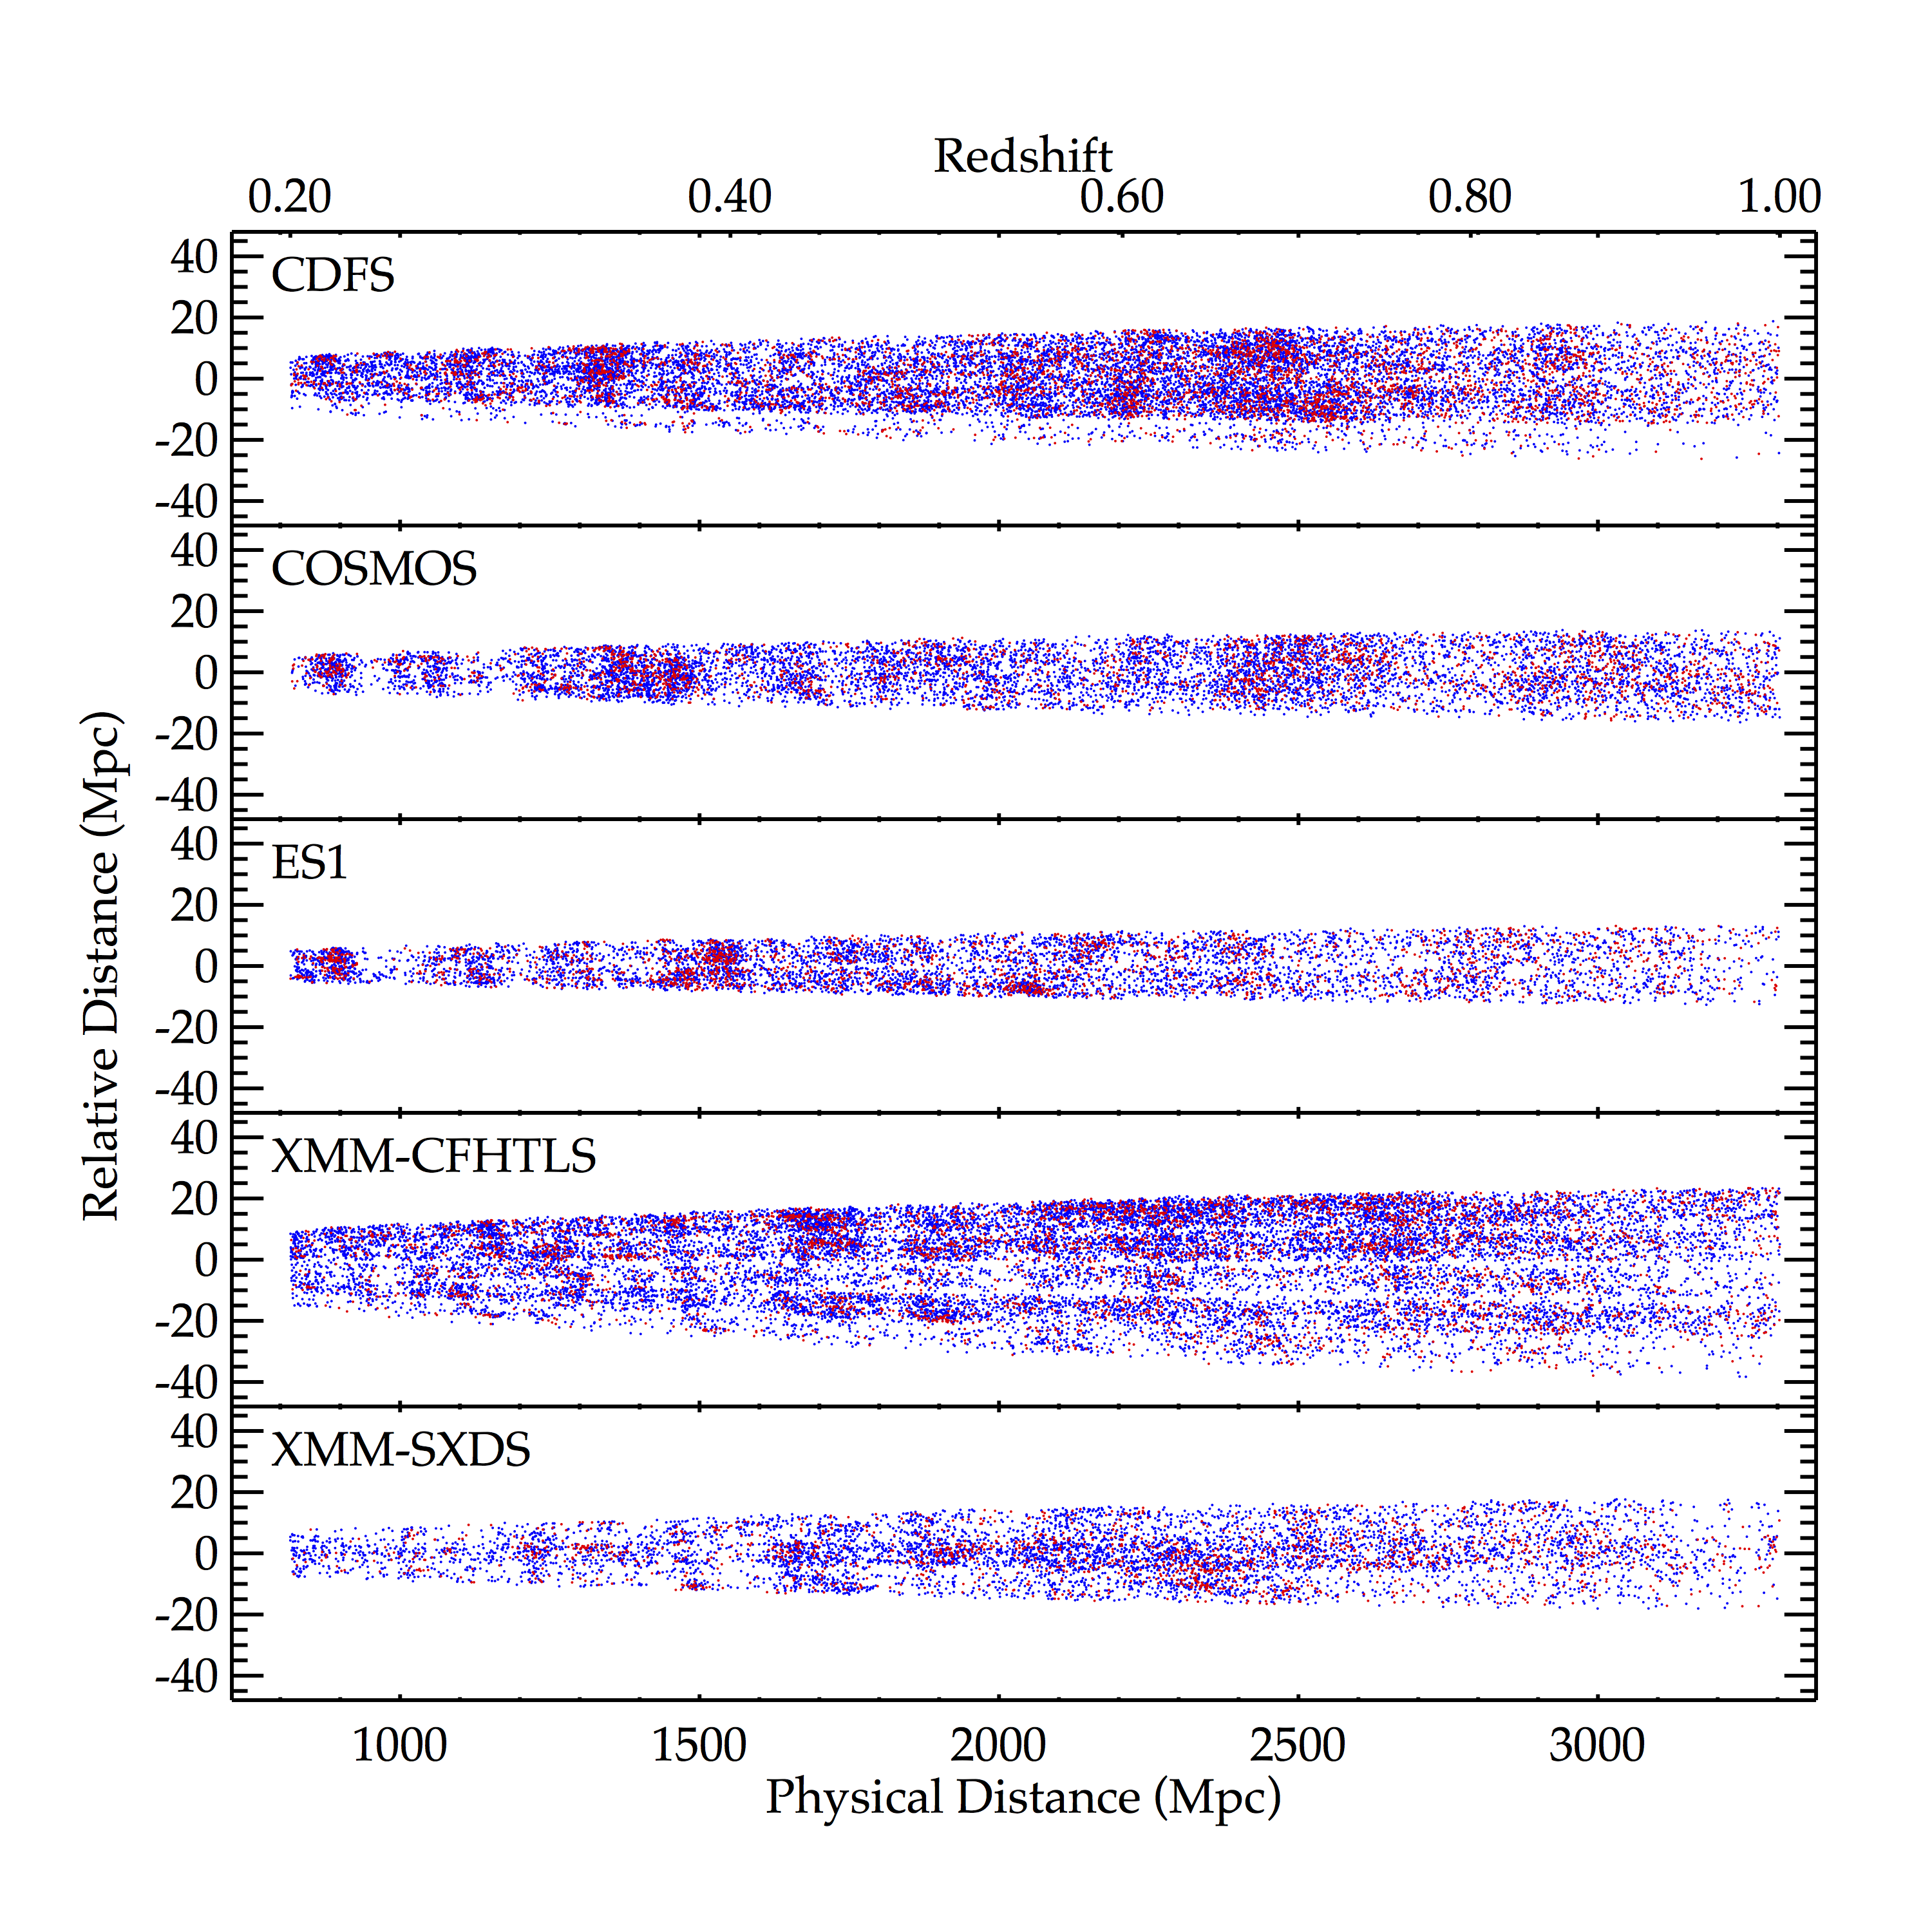
\includegraphics[width=0.9\textwidth,natwidth=600,trim={0.2in 0.5in 0.4in 0.6in},clip]{figures/cone_diagrams.png}}
  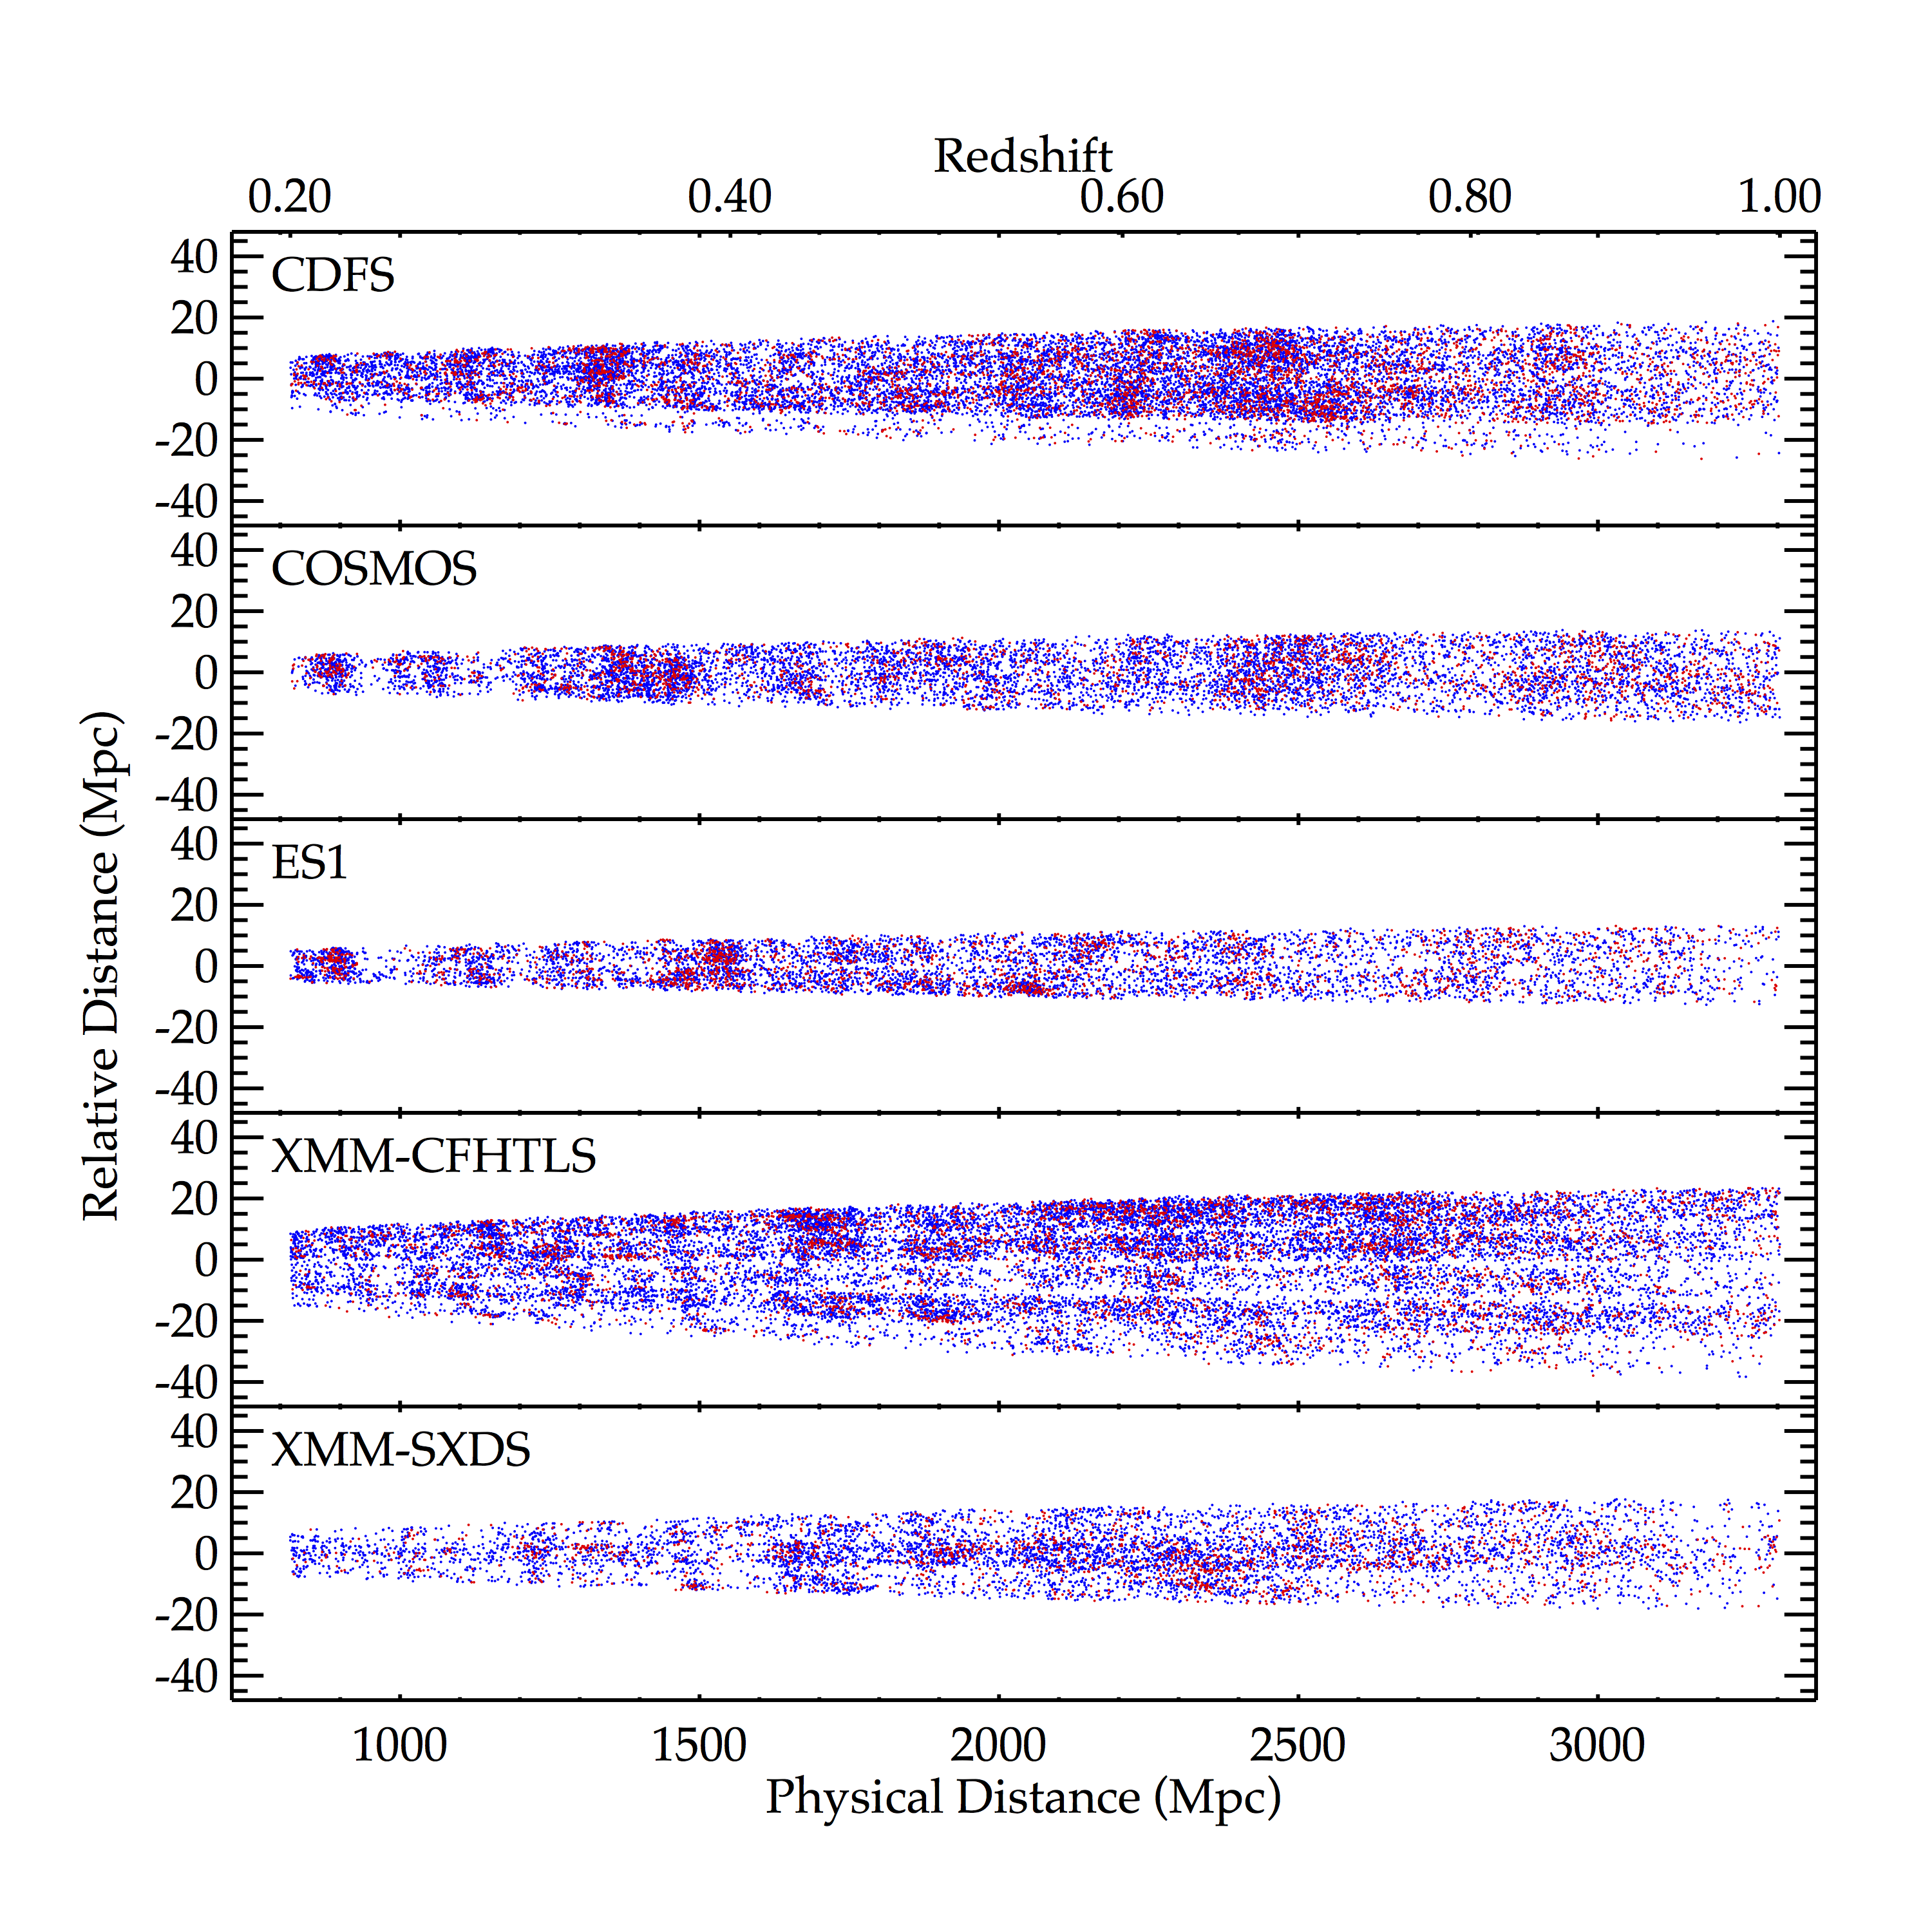
\includegraphics[width=0.8\textwidth,natwidth=600,trim={0.2in 0.5in 0.4in 0.6in},clip]{figures/cone_diagrams.png}
  \caption{Redshift space distributions of PRIMUS galaxies as a function of physical distance along the line-of-sight and right ascension 
(RA), relative to 
the median RA of the field.
%From top to bottom the corresponding fields are CDFS, COSMOS, ES1, XMM-CFHTLS, and XMM-SXDS.
Only galaxies with robust redshifts ${(Q \ge 3)}$ are shown.
Star-forming galaxies are shown in blue and quiescent galaxies in red (see~\S\ref{sec:SFQ}). Large scale differences in the observed 
density of galaxies, 
for example, as a function of RA, reflect the number of slitmasks and targeting density.
}
  \label{fig:cone_diagrams}
\end{figure*}

\subsection{Full Sample and Targeting Weights}\label{sec:targ_weight}
 

Objects in PRIMUS are classified as galaxies, stars, or broad-line active galactic nuclei by fitting the low-resolution spectra and multi-wavelength photometry 
for each source with an empirical library of templates.
The best-fit template defines both the redshift and the type of source.  
We exclude AGN from this study and keep only those objects defined as galaxies with robust redshifts {($Q\ge 3$)} in the redshift range ${0.2<z<1.0}$.
We also only keep galaxies with well defined targeting weights (these are termed ``primary'' galaxies in \citet{Coil11}; we do not use that naming here, to avoid 
confusion with our isolated primary sample defined below in \S\ref{sec:IPsample}).
These galaxies have a well understood spatial and targeting selection function, defined by both a density-dependent weight and a magnitude-dependent sparse-sampling 
weight, from which a statistically complete galaxy sample can be created.

PRIMUS targeting weights are described in detail in \citet{Coil11} and \citet{Cool13}.
% DENSITY-DEPENDENT WEIGHT
Briefly, density-dependent weights account for sources that PRIMUS could not target in dense survey regions, as galaxies are sufficiently clustered in the 
plane of
the sky to the PRIMUS flux limit that even two slitmasks per pointing could not target every galaxy below the magnitude limit in each field (as spectra would overlap on the detector). 
% MAGNITUDE-DEPENDENT "SPARSE SAMPLING WEIGHT"
Sparse-sampling weights are magnitude dependent and ensure that the PRIMUS target catalog is not dominated by the faintest objects within the survey flux limit. Sparse-sampling weights were used to randomly select roughly a third 
of galaxies in the faintest 0.5~mag interval above the primary sample 
targeting limit.
%Targets below the 100\% sampling limiting magnitude in each field (generally $i=22.5$) have a sparse-sampling weight of 1, while targets up to 0.5~mag fainter than 
%this limit (generally $22.5<i<23$) have a sparse-sampling weight of 0.3.
% REDSHIFT SUCCESS WEIGHT
A third, post-targeting weight \citep[detailed in][]{Cool13} accounts for the fact that not all PRIMUS spectra yielded reliable {($Q \ge 3$)} redshifts.
The average redshift success rate of the survey is a function of magnitude, declining from $>$75\% at ${i\le21}$ to $\sim$30\% at the survey limit of $i=23$, and is not a strong function of color.  
Taken together, these three weights allow for the recovery of a statistically complete galaxy sample from the targeted sources with reliable redshifts.  

The full sample used here includes 60,071 galaxies with robust redshifts between $0.2<z<1.0$ and well understood selection weights, in the five fields discussed above.
Below we test the sensitivity of our results to these targeting and completeness weights.

\subsection{Stellar Mass and SFR Estimates}\label{sec:SFR}
 
Stellar masses and star formation rates (SFRs) of PRIMUS galaxies are obtained with SED fitting, a widely adopted method for estimating the physical properties of galaxies.
A complete description of the SED fitting process using \iSEDfit can be found in \citet{Moustakas13}, but we summarize the relevant points here.
\iSEDfit is a suite of routines written in the \IDL programming language that uses galaxy redshifts and photometry to compute the statistical likelihood of a large ensemble of model SEDs for each galaxy.
Model SEDs are generated using population synthesis models, and span a wide range of observed colors and physical properties (age, metallicity, star formation history, dust content, etc.).
\iSEDfit uses a Monte Carlo technique to randomly select values of model parameters from user-defined parameter distributions and compute a posterior probability distribution function (PDF).
PDFs of stellar mass and SFR are the found by marginalizing over all other parameters, and the median value of the marginalized PDF is taken as the best estimate of the stellar mass or SFR of each galaxy.
%Uncertainties are taken to be one quarter of the 2.3 to 97.7 percentile range of the PDF, equivalent to a $1\sigma$ uncertainty in the case of a Gaussian distribution.

\subsection{Identifying Star-forming and Quiescent Galaxies}\label{sec:SFQ}

We divide our sample into star-forming and quiescent galaxies based on each galaxy's position in the SFR\textendash stellar mass plane. 
%relative to the star formation (SF) sequence \citep{Noeske07}, the correlation between SFR and stellar mass exhibited by star-forming galaxies to at least ${z\sim2}$ \citep{Oliver10; Karim11}.
Figure~\ref{fig:SFR_vs_mass} shows SFR versus stellar mass in six redshift bins from ${z=0.2}$--1 for the PRIMUS galaxy sample.
The dashed line (Eq.~\ref{eq:SFR}) in each panel traces the minimum of the bimodal galaxy distribution in that bin and is given by the following linear relation:
\begin{equation}
\log\,({\rm SFR}) = -1.29 + 0.65\,\log\,(\mass - 10) + 1.33\,(z - 0.1)
\label{eq:SFR}
\end{equation}

\noindent where SFR has units of $\sfrunit$ and $\mass$ has units of $\msun$.
The slope of this line is defined by the slope of the star forming main sequence \citep{Noeske07} as measured in the PRIMUS dataset using \iSEDfit SFR and stellar mass estimates. 
Each galaxy is classified as star-forming or quiescent based on whether it lies above or below the cut defined by Equation~\ref{eq:SFR}, evaluated at the redshift of the galaxy.

\begin{figure}
  \centering
%  \fbox{\includegraphics[width=\linewidth,natwidth=600,trim={0.1in 0.1in 0.2in 0.6in},clip]{figures/SFR_vs_mass}}
  \includegraphics[width=\linewidth,natwidth=600,trim={0.1in 0.1in 0.2in 0.6in},clip]{figures/SFR_vs_mass}
%  \epsscale{1.1}
%  \epstrim{0.1in 0.1in 0.2in 0.6in}
%  \fbox{\plotone{figures/SFR_vs_mass}}
%  \plotone{figures/SFR_vs_mass}
  \caption{Star formation rate (SFR) versus stellar mass for PRIMUS galaxies in six redshift bins from ${z=0.2}$--1.
Galaxies in our sample are classified as star-forming or quiescent according to whether they lie above or below the dashed line, respectively.
This line runs parallel to the star forming main sequence, traces the minimum in the galaxy SFR bimodality, and evolves with redshift according to Equation~\ref{eq:SFR}.
}
  \label{fig:SFR_vs_mass}
\end{figure}


\subsection{Isolated Primary Sample}\label{sec:IPsample}

In order to measure the galactic conformity signal, we must first identify isolated galaxies around which to search for the signal.
We follow \citet{Kauffmann13}, who selected in SDSS a volume-limited sample of galaxies with $\log\,\mstar>9.25$ and $0.017<z<0.03$.  They then defined ``central" galaxies of stellar mass $\mstar$ as those in their sample with no other galaxy with stellar mass greater than $\mstar/2$ within a projected radius of 500~kpc and with velocity difference less than 500~\kms.  Any galaxy in the full sample (defined above) is considered an isolated primary (IP) if there are no other galaxies
(i) within a projected physical distance of 500~kpc from the IP candidate,
(ii) within ${\pm 2.0\,\sigma_{z}\,(1 + z_{\rm IP})}$ in redshift space from the IP candidate (this includes as many true neighbors as possible while simultaneously minimizing interlopers and integrates over peculiar velocities), and
(iii) with stellar mass greater than half the stellar mass of the IP candidate.
Additionally, IPs can be neighbors of other IPs, and all galaxies can be a neighbor of multiple IPs. 

It is possible for galaxies near the edge of the survey area to be incorrectly classified as isolated if they have a sufficiently massive neighbor within a projected physical distance of 500~kpc that lies outside the survey area.
This could lead to contamination of our IP samples.
To test for this potential effect we visually inspected the distribution of IPs near the survey edges and concluded that false detections near edges do not significantly impact our IP sample, in that the spatial distribution of IPs does not rise substantially at the survey edges. 

\subsubsection{Stellar Mass Completeness Limits}\label{sec:mass_limit}

Because PRIMUS is a flux limited survey targeted in the $i$ band, galaxies with higher SFRs (i.e.~bluer galaxies) can be more easily detected at lower stellar mass than galaxies with lower SFR (i.e.~redder galaxies).
This introduces a bias towards star forming galaxies in the PRIMUS sample at lower stellar masses.
To account for this bias we define a stellar mass limit above which at least 95\% of all galaxies can be detected, regardless of their SFR.
This stellar mass completeness limit is a function of redshift, galaxy type (star-forming or quiescent), and also varies slightly between fields (due to the different photometry used for targeting in each field).
Details of the calculation of PRIMUS mass completeness limits can be found in \citet{Moustakas13}.
Briefly, we compute the stellar mass each galaxy would have if its apparent magnitude were equal to the survey magnitude limit, $\mlim$.  We then construct the cumulative distribution of $\mlim$ for the 15\% faintest galaxies in redshift bins of width 0.04, and calculate the minimum stellar mass that includes 95\% of the objects.  The limiting stellar mass versus redshift is fit with a separate quadratic polynomial for all, star-forming, and quiescent galaxies, and the fit is evaluated at the center of each redshift interval \citep[see][]{Moustakas13}.

In addition to the isolation criteria described above, all IPs must have stellar masses above the stellar mass completeness threshold specific to the galaxy's field, redshift, and type (star-forming or quiescent; see Table~\ref{table:mass_comp_limit}).  When identifying IPs, for each field and each redshift range in Table~\ref{table:mass_comp_limit} we eliminated any star-forming (quiescent) galaxy with stellar mass below the limiting value for star-forming (quiescent) galaxies in that field and redshift range.

Of the 60,071 galaxies in the full sample, 14,888 star-forming and 6,847 quiescent galaxies meet the isolation and stellar mass completeness criteria to be IPs.

\setlength{\tabcolsep}{0.02in}
\begin{deluxetable}{cccccc}
\tablecaption{Stellar mass completeness limits for star-forming and quiescent galaxies as a function of redshift.  At least 95\% of all galaxies above these stellar mass limits can be detected regardless of SFR.
\label{table:mass_comp_limit}}
\tablewidth{0pt}
\tablehead{
\colhead{}	&									
\colhead{\scriptsize CDFS}	&
\colhead{\scriptsize COSMOS}	&
\colhead{\scriptsize ES1}	&
\colhead{\scriptsize XMM-CFHTLS} &
\colhead{\scriptsize XMM-SXDS} \\
\cline{2-6} \\										
\colhead{Redshift Range} &
\multicolumn{5}{c}{$\log\,(\mlim/\msun)$}
}
\startdata
\multicolumn{6}{c}{Star-Forming} \\
\cline{1-6} \\[-1ex]
$0.20-0.30$ &	9.60	&	8.68	&	9.58	&	8.80	&	8.79	\\
$0.30-0.40$ &	9.92	&	9.05	&	9.94	&	9.06	&	9.13	\\
$0.40-0.50$ &	10.19	&	9.38	&	10.25	&	9.30	&	9.44	\\
$0.50-0.65$ &	10.44	&	9.75	&	10.59	&	9.58	&	9.77	\\
$0.65-0.80$ &	10.63	&	10.12	&	10.90	&	9.89	&	10.10	\\
$0.80-1.00$ &	10.69	&	10.46	&	11.14	&	10.21	&	10.38	\\
\cutinhead{Quiescent}										
$0.20-0.30$ &	9.65	&	9.23	&	9.80	&	9.17	&	9.35	\\
$0.30-0.40$ &	9.92	&	9.58	&	10.06	&	9.52	&	9.61	\\
$0.40-0.50$ &	10.17	&	9.89	&	10.30	&	9.85	&	9.85	\\
$0.50-0.65$ &	10.44	&	10.22	&	10.55	&	10.22	&	10.13	\\
$0.65-0.80$ &	10.71	&	10.52	&	10.79	&	10.60	&	10.43	\\
$0.80-1.00$ &	10.96	&	10.75	&	10.99	&	10.96	&	10.73	\\
\enddata
\end{deluxetable}


\subsubsection{Matching Stellar Mass and Redshift}\label{sec:IPsample_matching}

While our star-forming and quiescent IP populations are statistically complete (after applying the targeting and completeness weights), even above the stellar mass completeness limits the median stellar masses and redshifts of the two populations differ, as the stellar mass functions of star-forming and quiescent galaxies are different.
Figure~\ref{fig:IPhist_latefrac_vs_z} shows the redshift distributions of all star-forming (solid blue line) and quiescent (dashed red line) IPs, and the late-type fraction of all PRIMUS galaxies in the full sample as a function of redshift.
Our star-forming and quiescent IP populations have median stellar mass of $\log\,(\mstar/\msun)=10.44$ and 10.86, respectively, and median redshifts of $z=0.55$ and 0.60.

\begin{figure}
  \epsscale{1.1}
  \epstrim{0.1in 0.1in 0.5in 0.8in}
%  \fbox{\plotone{figures/IPhist_latefrac_vs_z}}
  \plotone{figures/IPhist_latefrac_vs_z}
  \caption{Top panel: Redshift histograms of all star-forming (solid blue line) and quiescent (dot-dashed red line) IPs.
Bottom panel: Late-type fraction of all PRIMUS galaxies in the full sample as a function of redshift. 
}
  \label{fig:IPhist_latefrac_vs_z}
\end{figure}

As discussed below, to compare the late-type fraction of neighbors around star-forming and quiescent IP galaxies we require the star-forming and quiescent IP samples to have the same stellar mass and redshift distributions.
To obtain these ``matched'' IP samples, we first apply to our IP samples an {\it upper} stellar mass cut derived from the PRIMUS stellar mass function (SMF, denoted as $\Phi$) for star-forming galaxies \citep{Moustakas13}.
This upper cut is required as there are fewer star-forming galaxies at high stellar mass ($\log\,(\mstar/\msun)>11$) than quiescent galaxies.
Therefore the high mass end of the star-forming galaxy SMF defines the limit of our matched IP samples.  
Specifically, we eliminate all IPs (both star-forming and quiescent) with stellar masses greater than the stellar mass at which 
${\log\,(\Phi \,/\, 10^{-4}\,\text{Mpc}^{-3}\,\text{dex}^{-1}) \le -3.7}$, interpolated at the redshift of each galaxy.
These upper mass limits are listed in Table~\ref{table:SMFlimit}.

%!TEX root = ../main.tex
\setlength{\tabcolsep}{0.1in}
\begin{deluxetable}{cc}
\tablewidth{0pc}
\tablecolumns{2}
\tablecaption{Matched IP sample stellar mass upper limits.
%$\log\,(\mlim/\msun)$ is the stellar mass in each redshift range where ${\log\Phi=-3.7}$.
%\tablenotemark{a}
\label{table:SMFlimit}
}
\tablehead{
%\multicolumn{1}{c}{} & \multicolumn{4}{c}{Area [deg$^2$]} & \multicolumn{6}{c}{Sample Size} \\
\colhead{Redshift Range} & \colhead{$\log\,(\mmax / \msun)$} }
\label{table:SMFlimit}
\startdata
$0.20-0.30$ & 11.154 \\
$0.30-0.40$ & 11.208 \\
$0.40-0.50$ & 11.255 \\
$0.50-0.65$ & 11.241 \\
$0.65-0.80$ & 11.308 \\
$0.80-1.00$ & 11.324 \\
%\hline \\[-2ex]
\enddata
%\tablenotetext{a}{$\mlim$ is the stellar mass in each redshift range where ${\log\Phi=-3.7}$.}
\end{deluxetable}


We then create a two-dimensional histogram of the stellar mass and redshift distribution of the remaining quiescent IP population, in bins of 0.2~dex in stellar mass and 0.05 in redshift.
For each of our five fields, in each bin we randomly select with replacement the same number of star-forming as there are quiescent IPs.
This selection is done separately in each field to account for field-to-field variations in the stellar mass and redshift distributions of the IP populations.
Our final matched IP sample (hereafter ``matched sample'') contains 6,197 unique quiescent and 4,185 unique star-forming IPs.
Each star-forming IP is assigned a weight equal to the number of times it was randomly selected while matching the distribution of the quiescent IP sample.
The sum of all star-forming IP weights therefore equals the total number of unique quiescent IPs.
Figure~\ref{fig:IPsample_matched} shows the stellar mass and redshift distributions of all star-forming and quiescent IPs in the full sample, as well as the stellar mass and redshift distributions of our matched sample.

\begin{figure}
  \epsscale{1.1}
  \epstrim{0.4in 0.2in 0.2in 0.4in}
%  \fbox{\plotone{figures/matchedSamplePlot_allFields}}
  \plotone{figures/matchedSamplePlot_allFields}
  \caption{Stellar mass and redshift distribution for all star-forming (blue solid contours) and quiescent (red dashed contours) IPs in the full sample. 
Gray shaded contours show the matched sample, in which star-forming and quiescent IPs have the same stellar mass and redshift distributions.
} 
  \label{fig:IPsample_matched}
\end{figure}

%FIELD	MAX WGT	weight fraction = 1
%cdfs		6	0.658472
%XMM-CFHTLS	7	0.691321
%cosmos		6	0.651163
%es1		7	0.623077
%xmm-sxds	9	0.676667


%!TEX root = main.tex

\section{Results}\label{sec:results}

In this section we discuss the importance of matching star forming and quiescent IP 
samples in both stellar mass and redshift, and we present the one- and two-halo 
conformity signal in the matched PRIMUS sample.  We discuss the effects of 
cosmic variance on measures of conformity and the need for jackknife
errors at intermediate redshifts, and we investigate the redshift and stellar mass 
dependence of conformity within the PRIMUS sample.

%\subsection{Neighbor Star-forming Fractions}\label{sec:LTfraction}
\subsection{The Effects of Matching Redshift and Stellar Mass on the Conformity Signal}\label{sec:LTfraction}

As discussed above, galactic conformity is the observed tendency of neighbor 
galaxies to have the same star-formation type (star-forming or quiescent) 
as their associated IP galaxy.
One-halo conformity refers to conformity between an IP and the neighbors within the 
same dark matter halo (i.e.~within $\sim1$~Mpc of the IP),
while two-halo conformity refers to conformity between an IP and neighbors in other 
adjacent halos (i.e.~at distances greater than $\sim1$~Mpc from the IP).

We therefore want to measure how the fraction of neighbors that are star-forming differs 
between star-forming and quiescent IP hosts as a function of projected radius from 
the IP.
To do this, for each IP in our matched sample we count all neighbors within 
concentric cylindrical shells of length ${2\times2\,\sigma_{z}(1+z_{\text{IP}})}$
and cross-sectional area
${\pi[(\Rproj+d\Rproj)^2-\Rproj^2]}$, where $\Rproj$ is the 2D projected radius from the IP in (physical) Mpc, and $d\Rproj$ is the shell width in Mpc.
The star-forming fraction of neighbors of star-forming IPs in a cylindrical shell 
at projected radius $\Rproj$ to ${(\Rproj+d\Rproj)}$, $f^{\textrm{SF-IP}}_{\textrm{SF}}
(\Rproj)$ is defined to be the sum of the targeting weights (see~\S\ref{sec:targ_weight}) of the star-forming neighbors of star-forming IPs in the shell, 
divided by the sum of the
targeting weights of \emph{all} neighbors of star-forming IPs in the shell:
\begin{equation}
        f^{\textrm{SF-IP}}_{\textrm{SF}}(\Rproj) = \frac
        {\displaystyle \sum_{i=1}^{N_{\textrm{SF-IP}}} \sum_{j=1}^{N_{\textrm{SF},i}} w_{ij} }
        {\displaystyle \sum_{i=1}^{N_{\textrm{SF-IP}}} \sum_{k=1}^{N_{\textrm{tot},i}} w_{ik} },
\label{eq:SFfrac}
\end{equation}
and likewise for quiescent IPs.
$N_{\textrm{SF-IP}}$ is the total number of star-forming IPs, $N_{\textrm{SF},i}$ is the number of star-forming neighbors of IP $i$ in the shell, $N_{\textrm{tot},i}$ is the
total number of neighbors of IP $i$ in the shell, and $w_{ij}$ and $w_{ik}$ are PRIMUS targeting weights of the neighbors.
We are therefore essentially computing neighbor star-forming fractions for star-forming 
and quiescent IPs by stacking the neighbors of all IPs of each type.

\begin{figure*}
  \epsscale{0.85}
  \epstrim{0.1in 0.3in 0.4in 0.8in}
%  \fbox{\plotone{figures/unmatchedIPsampleCompare}}
  \plotone{figures/unmatchedIPsampleCompare}
  \caption{
The fraction of star-forming neighbor galaxies around star-forming 
and quiescent IPs, to a projected distance of ${\Rproj<15}$~Mpc, 
 for four different IP samples: 
(a)~all IP candidates above the M13 mass completeness limit (\S\ref{sec:mass_limit});
(b)~IP candidates that also have the same redshift distribution for the star-forming
and quiescent IPs; 
(c)~IP candidates that have the same stellar mass distribution;
(d)~IPs that have both matched stellar mass and redshift distributions.
The median redshift and stellar mass of each IP sample are shown in each panel.
}
  \label{fig:IPsample_compare}
\end{figure*}


The importance of matching both the stellar mass and redshift distributions of our 
IP sample is clearly illustrated in Figure~\ref{fig:IPsample_compare}, which shows 
how the star-forming fractions of neighbors around star-forming and quiescent IPs 
differ when different IP samples are used.
Figure~\ref{fig:IPsample_compare} shows the fraction of neighbors of star-forming 
and quiescent IPs that are star-forming as a function of projected radius from the 
IP in 1~Mpc annuli out to 15~Mpc for four different IP samples.
%

In panel (a) all IP candidates above the M13 mass completeness limit 
(\S\ref{sec:mass_limit}) are included.
Here the median stellar mass of the quiescent IP population is 0.42~dex greater 
than that of the star-forming IP population, and the median redshift is greater 
by 0.05.
This difference in the stellar mass distribution in particular means that 
star-forming IPs are preferentially located at lower redshift, where the star-forming fraction of \emph{all} PRIMUS galaxies (the ``full'' sample; see~\S\ref{sec:targ_weight}) is larger than at higher redshifts.  The star-forming fraction of the full sample declines steadily from 0.80 at $z\sim0.2$ to 0.73 at $z\sim1.0$, causing us to overestimate of the neighbor star-forming fraction for star-forming IPs at all projected radii.
The result is a relatively fixed offset between the solid and dashed lines in the 
left panel of Figure~\ref{fig:IPsample_compare} that persists to the largest 
projected radii we measure with PRIMUS, mimicking a conformity signal.  We therefore
measure a ``false'' conformity signal in this sample.

In panel (b) we select star-forming and quiescent IP samples with matched redshift 
distributions using the method described in \S\ref{sec:IPsample_matching}.  This 
causes the large-scale offset to disappear, but there is still a difference in the 
median stellar masses of the IP samples of 0.3~dex.  Since star-forming fraction depends on stellar mass, that is not ideal. 
In panel (c) we select star-forming and quiescent IP samples with matched stellar mass distributions; this results in a star-forming IP sample with a higher median 
redshift than that of the quiescent IP sample (by 0.05).
In this case the systematic bias mimics the opposite of a conformity signal; the solid line moves closer to the dashed line at all projected radii, actually dropping below it at $>5$~Mpc.

Finally, panel (d) shows results for our matched stellar mass and matched redshift IP sample.
Failure to control for differences in the stellar mass and/or redshift distributions 
can introduce bias into the relative neighbor star-forming fractions of star-forming and quiescent IPs.
Only by matching both the stellar mass and redshift distributions of our star-forming and quiescent IP samples do we eliminate systematic biases in neighbor star-forming fraction measurements that could masquerade as a conformity signal.
For the remainder of this paper, the IP samples matched in both stellar mass and redshift are referred to as the ``matched'' sample.


\subsection{One- and Two-Halo Conformity Signal in Matched Sample}\label{sec:signal}

\begin{figure*}
  \epsscale{0.7}
  \epstrim{0.4in 0.1in 0.3in 0.4in}
%  \fbox{\plotone{figures/latefracplot_BSE_IPmatchFBF_PHI37_allz_250kpc}}
  \plotone{figures/latefracplot_BSE_IPmatchFBF_PHI37_allz_250kpc}
  \caption{
The fraction of star-forming neighbor galaxies around star-forming 
and quiescent IPs, to a projected distance of ${\Rproj<5}$~Mpc, 
for IP samples matched in both stellar mass and redshift, using 
finer ${d\Rproj=0.25}$~Mpc radial bins for all star-forming (blue solid line) and quiescent (red dashed line) IPs in the matched sample.
The errors shown have been computed by bootstrap resampling.
}
  \label{fig:latefrac_matched}
\end{figure*}

Stacked neighbor star-forming fractions for the matched sample of star-forming and quiescent IPs are shown in Figure~\ref{fig:latefrac_matched}, here using finer radial bins.  The errors here and above have been estimated by bootstrap resampling, where for each radial bin we randomly select with replacement 90 percent of all star-forming or quiescent IPs 200 times, and compute $\flate$ for each of the 200 samples.  The bootstrap error is the standard deviation of the $\flate$ distribution.  Below in \S\ref{sec:errors} we discuss the merits of estimating error with jackknife versus bootstrap resampling.

In Figure~\ref{fig:latefrac_matched} the one-halo component of the conformity signal is clearly visible as the 4--7\% difference between $\flate$ for star-forming and quiescent IPs at $\Rproj < 1$~Mpc.  Within this range, $\flate$ for both IP types is greatest at $\Rproj<0.5$~Mpc;~$\sim0.86$ for star-fomring and $\sim0.79$--0.82 for quiescent IPs.  At $\Rproj=0.5$~Mpc $\flate$ for both IP types drops sharply by at least 8\% to $\sim0.76$ for star-forming and $\sim0.72$ for quiescent IPs.

This break at 500~kpc is an artifact of the isolation criteria used to identify isolated primaries 
(see \S\ref{sec:IPsample}), and the fact that the fraction of all galaxies in our full sample that are
star-forming is a decreasing function of stellar mass.
Because we require IP galaxies (regardless of type) to have no other galaxies more massive than half the
stellar mass of the IP within 500 projected kpc, the median stellar mass of galaxies within 500~kpc will
automatically be lower than the median stellar mass of galaxies beyond this distance.
The star-forming fraction of neighboring galaxies within 500~kpc will therefore be greater than the star-forming
fraction of neighbors within $\Rproj=0.5$--5~Mpc.

To confirm that this feature of Figure~\ref{fig:latefrac_matched} is a direct result of our choice of a
projected radius of 500~kpc when identifying IPs, we also measured $\flate$ for redshift and stellar 
mass-matched samples of star-forming and quiescent IPs selected using 250 and 750~kpc as the projected 
radius in our isolation criteria.
As expected, when 250~kpc is used to identify IPs, the break in $\flate$ 
for both star-forming and quiescent IPs occurs at 250~kpc, and likewise for 750~kpc.
Because conformity is the \emph{difference} between $\flate$ for star-forming and quiescent IPs, and does
not depend on the absolute star-forming neighbor fraction for either IP type, this break at 500~kpc does
not affect our result.

Over $\Rproj\simeq1$--1.5~Mpc $\flate$ for quiescent IPs increases to $\sim0.75$, while for star-forming IPs $\flate$ begins to level off at $\sim0.76$.  This $\sim1$\% difference between the two fractions is a two-halo conformity signal that persists to to roughly 3~Mpc.  At $3\lesssim\Rproj<5$~Mpc $\flate$ for both IP types is effectively constant and nearly equal, such that no conformity signal is present beyond $\Rproj\simeq3$~Mpc.

%%%%%%% EQUAL WEIGHT TO EACH IP:

\begin{figure}
  \epsscale{1.1}
  \epstrim{0.5in 0.1in 0.3in 0.3in}
%  \fbox{\plotone{figures/latefracplot_BSE_IPmatchFBF_PHI37_allz_median_quartiles}}
  \plotone{figures/latefracplot_BSE_IPmatchFBF_PHI37_allz_median_quartiles}
  \caption{
Similar to Figure~\ref{fig:latefrac_matched}, except here $\flate$ is the median of 
the distribution of non-zero individual neighbor star-forming fractions for each IP type as a function of $\Rproj$.  This effectively gives equal weight to each IP, instead of upweighting the IPs with more neighbors, as shown in Figure 6.
Also shown here is the mean of the non-zero neighbor star-forming fraction distributions of star-forming and quiescent IPs (purple dot-dashed and magenta dotted lines),
and the interquartile range of the combined distribution for both IP types (gray shaded region).
}
  \label{fig:latefrac_quartiles}
\end{figure}

Within a particular radial bin (or shell around each IP), this stacking method 
weights IPs with more neighbors more heavily than those with fewer or no neighbors,
for that bin.
To assess whether this will bias our results, we recompute the neighbor star-forming fraction, 
now assigning equal weight to each IP by computing the star-forming fraction 
individually for each IP and then taking the median of the distribution of all 
non-zero fractions for both IP types, within each 1~Mpc radial bin.
The result is shown in Figure~\ref{fig:latefrac_quartiles}, which also shows the 
mean individual neighbor star-forming fraction for both IP types in each radial bin (again using
only non-zero fractions), and the interquartile range (25$^{\textrm{th}}$ to 75$^{\textrm{th}}$ percentile) of the combined $\flate$ distribution for both IP types.

Above $\Rproj=1$~Mpc the large spread in the interquartile range indicates that three quarters of IPs have a neighbor star-forming fraction of at least 65\%, while for one quarter of IPs the star-forming fraction is over 90\%.
Median and interquartile range values are not shown for $\Rproj=0$--1~Mpc because in this bin the median (and 75$^{\textrm{th}}$ percentile) value of $\flate$ for both IP types is 1.

In the $\Rproj<1$~Mpc bin the only meaningful measure of conformity is the mean values of the $\flate$ distributions.
Comparing the mean values we observe a conformity signal of a few percent at $\Rproj<1$~Mpc.
Both the mean and median exhibit a smaller signal of $\sim1$--2\% at $1<\Rproj<3$~Mpc, and no signal at projected radii greater than 3~Mpc.

The difference between neighbor star-forming fractions for star-forming and quiescent IPs is comparable for equal weighting of IPs as shown here and when each IP is weighted proportionally to its number of neighbors, as shown in Figure~\ref{fig:latefrac_matched}.

\setlength{\tabcolsep}{0.03in}
%\begin{deluxetable*}{cccccccccccc}[!h]
\begin{deluxetable*}{ccrrrcccrcccrcc}
\tabletypesize{large}
\tablecaption{Conformity Signal (Jackknife Errors)\label{table:signal}}
\tablewidth{0pt}
\tablehead{
\multicolumn{2}{c}{$N_{\textrm{IP}}$} & \colhead{} & \colhead{} &
\multicolumn{3}{c}{$0.0 < R < 1.0$~Mpc} & {} &
\multicolumn{3}{c}{$1.0 < R < 3.0$~Mpc} & {} &
\multicolumn{3}{c}{$3.0 < R < 5.0$~Mpc} \\
\cline{1-2}\cline{5-7}\cline{9-11}\cline{13-15} \\
\colhead{SF} & \colhead{Q} &
\multicolumn{1}{c}{$z$} &
\multicolumn{1}{c}{$\log\,(\mstar/\msun)$} &
\colhead{$\signorm$} & \colhead{$\sigma_{\textrm{JK}}$} & \colhead{($\sigma_{\textrm{BS}}$)} & {} &
\colhead{$\signorm$} & \colhead{$\sigma_{\textrm{JK}}$} & \colhead{($\sigma_{\textrm{BS}}$)} & {} &
\colhead{$\signorm$} & \colhead{$\sigma_{\textrm{JK}}$} & \colhead{($\sigma_{\textrm{BS}}$)} \\
\cline{1-15} \\
\multicolumn{15}{c}{Full Sample}
}
\startdata
$4,185$ &
$6,197$ &
[0.20, 1.00] &
[9.13, 11.33] &
$0.053\pm0.015$ & 3.6 & $(6.8)$  & {} &
$0.009\pm0.004$ & 2.5 & $(3.9)$  & {} &
$-0.003\pm0.004$ & 0.7 & $(1.3)$  \\
\cutinhead{Redshift Bins}
$2,241$ &
$3,096$ &
[0.20, 0.59] &
[9.13, 11.25] &
$0.052\pm0.013$ & 4.0 & $(4.9)$  & {} &
$0.007\pm0.004$ & 1.9 & $(2.3)$  & {} &
$-0.005\pm0.006$ & 0.9 & $(1.8)$  \\
$1,945$ &
$3,101$ &
[0.59, 1.00] &
[10.11, 11.33] &
$0.056\pm0.026$ & 2.1 & $(4.5)$  & {} &
$0.014\pm0.007$ & 2.0 & $(3.6)$  & {} &
$0.002\pm0.006$ & 0.4 & $(0.6)$  \\
\cline{1-15} \\
$1,520$ &
$2,047$ &
[0.20, 0.48] &
[9.13, 11.25] &
$0.061\pm0.012$ & 5.1 & $(5.1)$  & {} &
$0.009\pm0.005$ & 1.7 & $(2.4)$  & {} &
$-0.005\pm0.007$ & 0.8 & $(1.4)$  \\
$1,406$ &
$2,086$ &
[0.48, 0.68] &
[9.92, 11.28] &
$0.043\pm0.025$ & 1.7 & $(3.0)$  & {} &
$0.001\pm0.006$ & 0.2 & $(0.3)$  & {} &
$-0.002\pm0.005$ & 0.5 & $(0.7)$  \\
$1,261$ &
$2,064$ &
[0.68, 1.00] &
[10.31, 11.33] &
$0.048\pm0.041$ & 1.2 & $(2.7)$  & {} &
$0.023\pm0.010$ & 2.2 & $(4.2)$  & {} &
$0.004\pm0.008$ & 0.5 & $(0.7)$  \\
\cutinhead{Stellar Mass Bins}
$2,385$ &
$3,069$ &
[0.20, 1.00] &
[9.13, 10.82] &
$0.039\pm0.013$ & 2.9 & $(3.7)$  & {} &
$0.005\pm0.004$ & 1.2 & $(1.6)$  & {} &
$0.000\pm0.004$ & 0.1 & $(0.1)$  \\
$1,801$ &
$3,128$ &
[0.20, 1.00] &
[10.82, 11.33] &
$0.070\pm0.021$ & 3.3 & $(5.9)$  & {} &
$0.014\pm0.004$ & 3.3 & $(3.9)$  & {} &
$-0.008\pm0.006$ & 1.3 & $(2.2)$  \\
\cline{1-15} \\
$1,649$ &
$2,064$ &
[0.20, 0.80] &
[9.13, 10.67] &
$0.051\pm0.015$ & 3.4 & $(3.8)$  & {} &
$0.002\pm0.005$ & 0.3 & $(0.5)$  & {} &
$-0.004\pm0.005$ & 0.8 & $(1.0)$  \\
$1,410$ &
$2,019$ &
[0.20, 1.00] &
[10.67, 10.95] &
$0.024\pm0.019$ & 1.3 & $(1.9)$  & {} &
$0.013\pm0.005$ & 2.5 & $(3.0)$  & {} &
$-0.002\pm0.004$ & 0.6 & $(0.6)$  \\
$1,126$ &
$2,113$ &
[0.21, 1.00] &
[10.95, 11.33] &
$0.089\pm0.020$ & 4.4 & $(5.9)$  & {} &
$0.015\pm0.007$ & 2.3 & $(3.4)$  & {} &
$-0.004\pm0.007$ & 0.6 & $(0.9)$  \\
\enddata
\end{deluxetable*}



%%%%%%%%%  NORMALIZED CONFORMITY SIGNAL:

To better quantify our results we define the normalized conformity signal, 
$\signorm$, at a projected radius of $\Rproj$ as the difference of the neighbor star-forming fractions of star-forming and quiescent IPs, 
divided by the mean of these two fractions:

\begin{equation}
	\signorm(\Rproj) = \frac
	{ f^{\textrm{SF-IP}}_{\textrm{SF}}-f^{\textrm{Q-IP}}_{\textrm{SF}} }
	{ \left( f^{\textrm{SF-IP}}_{\textrm{SF}}+f^{\textrm{Q-IP}}_{\textrm{SF}} \right) /2}
\label{eq:signorm}
\end{equation}

Table~\ref{table:signal} presents the 
normalized conformity signal in the matched sample in integrated radial bins of 
{${\Rproj=0}$--1}, {1--3}, and {3--5~Mpc}.
Over the full redshift range ${0.2<z<1.0}$ we find a normalized one-halo conformity 
signal of 5.3\% and a two-halo signal of 1.1\%.
We emphasize that galactic conformity is a very small effect, especially the two-halo term, making it highly sensitive to observational uncertainty.
Galactic conformity therefore cannot be accurately measured without a sufficiently large sample volume.
The above measurements were made using a sample of over 60,000 galaxies in a ${2.94\times10^7}$~Mpc$^3$ volume spanning over 5~Gyr of cosmic time from $z=0.2$--1.
The observed density of galaxies in our full sample is ${2\times10^{-3}}$~Mpc$^{-3}$.

\begin{figure}
  \epsscale{1.1}
  \epstrim{0.3in 0.1in 0.2in 0.3in}
%  \fbox{\plotone{figures/normsigplot_allz_errorCompare}}
  \plotone{figures/normsigplot_allz_errorCompare}
  \caption{Normalized conformity signal, $\signorm$, for the matched sample measured to ${\Rproj<5}$~Mpc, with both bootstrap (orange) and jackknife errors (black) shown.  The jackknife errors exceed the bootstrap errors by up to a factor of $\sim2$.
}
  \label{fig:normsig_matched}
\end{figure}


\subsection{Bootstrap Versus Jackknife Errors}\label{sec:errors}

In Table~\ref{table:signal} we estimate the uncertainty in $\signorm$ using both bootstrap and jackknife resampling, and quote the significance we find using each 
method as $\sigmaBS$ and $\sigmaJK$, respectively.
We compute Bootstrap errors by selecting 90\% of the data randomly with replacement 200 times, and then taking the standard deviation of the 200 results.
To compute jackknife errors we divide the survey area of the matched sample into 10 regions of approximately $0.5~\degsq$ each.
We then compute $\signorm$ 10 times, systematically excluding one of the 10 jackknife samples each time, and take the standard deviation of the 10 results as the error.

Each method gives information about a different type of variation in our sample.
Bootstrap resampling provides an estimate of the variation of $\flate$ for the entire matched IP sample \emph{as a whole}.
It does not, however, take into account that our matched sample contains four spatially distinct fields of different sizes on the sky.

Jackknife resampling estimates the uncertainty in $\flate$ \emph{due to field-to-field variation} (i.e.~cosmic variance) within the matched sample.
As seen in Table~\ref{table:signal}, jackknife resampling yields errors that are at least as large as bootstrap errors at all projected radii,
and which usually exceed bootstrap errors by a factor of $\sim2$.
Cosmic variance is therefore the dominate source of uncertainty in our result.

We emphasize that any meaningful measurement of conformity at $z>0.2$ should accurately account for cosmic variance by using multiple spatially distinct fields and jackknife errors.
Bootstrap resampling is sufficient to estimate the uncertainty of a conformity signal \emph{within a single field}, but the result obtained with any one field cannot
realistically be extrapolated to draw conclusions about conformity on larger scales (see also \S\ref{sec:cosmic_var}).

Figure~\ref{fig:normsig_matched} shows $\signorm$ for the matched sample in ${d\Rproj=1}$~Mpc bins with both jackknife and bootstrap errors.
In the matched sample we find that for ${0<\Rproj<1}$~Mpc the bootstrap error of $\signorm$ is ${\pm0.008}$, which yields a significance of $\sigmaBS=6.8$, while the jackknife error is ${\pm0.015}$, with a significance of $\sigmaJK=3.6$.
 
The above result uses all star-forming and quiescent IPs in the matched sample, regardless of specific SFR (sSFR).  
To test whether the conformity signal is sensitive to the magnitude of the difference in sSFR between star-forming and quiescent IPs, we also measure one- and two-halo conformity with only the extreme high and low ends of the IP sSFR distribution.  Specifically, we compute $\signorm$ highest and lowest quartiles of IP sSFR (also matched in stellar mass and redshift distribution).

The one-halo term over the full redshift range increases slightly to 5.5\%, while the uncertainty decreases to 1.2\%.
This increases $\sigmaJK$ to 4.7, even though the sample is half the size of the matched IP sample.
The two-halo term increases slightly to 1.5\%, but the uncertainty also increases to 0.9\%, which decreases $\sigmaJK$ to from 2.5 to 1.7.

%{\bf(move this above to the results section - maybe the end of section 3.3 - not good to highlight our redshift errors here)}
Additionally, the ${\sigmaz/(1+z) = 0.005}$ PRIMUS redshift precision will result in a dilution of the 
true conformity signal, as there will be some contamination from satellite galaxies in our IP sample.
This implies that our measured conformity signal should be treated as a lower limit on the true signal.

\subsection{Cosmic Variance (Field-to-Field Variation?)}\label{sec:cosmic_var}

\begin{figure}
  \epsscale{1.1}
  \epstrim{0.4in 0.7in 0.3in 0.3in}
%  \fbox{\plotone{figures/normsigplot_byField_1halo}}
  \plotone{figures/normsigplot_byField_1halo}
  \caption{
One-halo term ($0<\Rproj<1$~Mpc) of $\signorm$ for each field and the matched sample.
Field errors are estimated by bootstrap resampling within the field, while the error signal measured with all fields is estimated by jackknife resampling.
}
  \label{fig:normsig_fields_1halo}
\end{figure}

\begin{deluxetable}{lrrr}
\tabletypesize{large}
\tablecaption{Signifcance of 1-halo conformity signal ($0<\Rproj<1$~Mpc) for individual fields.
\label{table:signal_fields}}
\tablewidth{0pt}
\tablehead{
\colhead{Field} & \colhead{$N_{\textrm{SF-IP}}$} & \colhead{$N_{\textrm{Q-IP}}$} & \colhead{$\sigma_{\textrm{BS}}$} \\
}
\startdata
CDFS &
$1,139$ &
$1,698$ &
$4.0$ \\
COSMOS &
$731$ &
$1,099$ &
$3.1$ \\
ES1 &
$390$ &
$621$ &
$5.9$ \\
XMM-CFHTLS &
$1,325$ &
$1,897$ &
$3.4$ \\
XMM-SXDS &
$600$ &
$882$ &
$0.2$ \\
\cline{1-4} \\
Full Sample ($\sigma_{\textrm{JK}}$) &
$4,185$ &
$6,207$ &
$3.6$ \\
\enddata
\end{deluxetable}


Errors estimated with jackknife resampling account for variation in the 
magnitude of the conformity signal among spatially distinct regions of the sky.
The fact that $\sigmaJK$ is significantly less than $\sigmaBS$ for every conformity signal measurement in Table~\ref{table:signal}
illustrates the importance of accounting for cosmic variance in any conformity measurement.

We further investigate how the conformity signal in PRIMUS is sensitive to cosmic variance by measuring the one-halo term of $\signorm$ {($0<\Rproj<1$~Mpc)} for each field individually.
The results are shown in Table~\ref{table:signal_fields} and Figure~\ref{fig:normsig_fields_1halo}.
The errors on the individual field measurements in Figure~\ref{fig:normsig_fields_1halo} are computed by bootstrap resampling within the field, and represent the uncertainty of the one-halo conformity signal \emph{in that field}.
The error on the one-halo signal measured over all five fields is computed by jackknife resampling from all fields, and represents the uncertainty of the matched sample one-halo term due to variation \emph{among} different fields.

The field-to-field variation within PRIMUS is substantial.
Among the five fields in the matched sample the one-halo term of 
$\signorm$ varies from over $12\%$ with $\sigmaBS=5.9$ in ES1, to $\sim5$\% in 
CDFS, COSMOS, and XMM-CFHTLS, to $0\%$ with $\sigmaBS\simeq0$ in XMM-SXDS.
This variation clearly indicates the importance of measuring conformity in multiple fields.  A large dispersion exists in the strength of conformity among PRIMUS fields, and the signal in any one field can differ significantly from the mean.


\subsection{Redshift and Stellar Mass Dependence}\label{sec:z_mass_bins}

H15b predicts that conformity strength (specifically two-halo) should decrease with both increasing central galaxy halo mass and increasing redshift, weakening significantly by $z\sim1$ and disappearing entirely by $z\sim2$.
With PRIMUS we can test for trends in conformity signal strength with redshift to $z=1$, and with halo mass using IP stellar mass as a proxy for halo mass.
We further divide the matched sample into two redshift bins and two stellar mass bins, 
to investigate the dependence in the magnitude of the signal on redshift or 
stellar mass.
In Figure~\ref{fig:latefrac_normsig_compare} we divide the matched IP sample into two redshift bins, ${0.2<z<0.59}$ and ${0.59<z<1}$, and two stellar mass bins, 
${\logM=9.13}$--10.82 and 10.82--11.33, each containing equal numbers of IPs.
The upper panels show $\flate$ for star-forming and quiescent IPs in each redshift or stellar mass bin, while the lower panels plot the corresponding values of
$\signorm$ for each radial bin. The normalized signal and significance are given in 
Table~\ref{table:signal}.

\begin{figure*}
  \epsscale{1.0}
  \epstrim{0.2in 0.3in 0.4in 0.8in}
%  \fbox{\plotone{figures/latefrac_normsig_binnedCompare}}
  \plotone{figures/latefrac_normsig_binnedCompare}
  \caption{
Top panels: Neighbor star-forming fractions for star-forming (solid and dash-dot blue lines) and quiescent (dashed red lines) IPs in our matched sample divided into two redshift bins (left) and two stellar mass bins (right).  Errors are computed by bootstrap resampling and have been offset for clarity.
Bottom panels: $\signorm$ for the corresponding redshift and stellar mass divisions in the top panels.  Errors are computed by jackknife resampling.
The bottom panels also show $\signorm$ for the higher redshift bin (left) and higher stellar mass bin (right) computed \emph{without} the COSMOS field (dashed gray line).
}
  \label{fig:latefrac_normsig_compare}
\end{figure*}

When dividing into redshift bins the one-halo term of $\signorm$ in both bins is comparable to the 5.3\% signal observed over the full redshift range.
The significance of the ``low'' redshift (${0.2<z<0.59}$) one-halo term increases to 
${\sigmaJK=4.0}$, while the significance of the ``high'' redshift one-halo term drops to ${\sigmaJK=2.1}$.
The magnitude of the two-halo term of $\signorm$ in each bin also remains comparable to the full redshift range signal of 1.1\%, but the uncertainty in each bin also increases,
reducing $\sigmaJK$ from 2.5 for the full redshift range to 1.7 and 1.6 for the low and high redshift bins, respectively.

Dividing the matched sample into two stellar mass bins, we find a significant ($\sim3\sigma$) increase of $\sim75\%$ in one-halo conformity strength for higher compared to lower stellar masses, and a similar although less significant trend with stellar mass in the two-halo term.
Specifically, the one-halo term drops to ${3.9(\pm1.3)}$\% for the low stellar mass bin (${9.13<\logM<10.82}$), but
increases to ${7.0(\pm2.1)}$\% for the high-mass bin (${10.82<\logM<11.33}$).
The low stellar mass two-halo term is ${0.8(\pm0.6)}$\% and increases to ${1.5(\pm0.5)}$\% for high stellar mass.

Assuming that galaxy stellar mass is tightly coupled with host halo mass, these results appear to contradict the H15b prediction that conformity strength should decrease with increasing halo mass.
However, the H15b prediction is specifically for two-halo conformity, where the significance of our result is lower.
Additionally, as we explain in the following section, field-to-field variation may have an important effect on the trends we observe.

%The most important conclusion is that a larger sample area spanning additional distinct fields is needed to robustly test predictions about the mass (and redshift) dependence of two-halo conformity.

\subsubsection{The Effect of the COSMOS Field}\label{sec:cosmos}

The COSMOS field contains a high degree of large-scale structure at $z\sim0.35$ and $z\sim0.7$, presenting another opportunity to test the impact of field-to-field variation on our results.
As Figure~\ref{fig:fig:normsig_fields_1halo} and Table~\ref{table:signal_fields} show, the one-halo conformity term in the COSMOS field alone agrees well with the one-halo term of the full matched sample.
However, we also measure the two-halo term (${1<\Rproj<3}$~Mpc) of $\signorm$ for each field individually, and found that it is stronger in COSMOS than in any other field.
Additionally, when we divide the matched sample into two redshift and two stellar mass bins, the two-halo term is stronger in both the higher redshift and higher stellar mass bin (see Figure~\ref{fig:latefrac_normsig_compare} and Table~\ref{table:signal}).

To investigate the degree to which COSMOS contributes to the higher redshift and high stellar mass two-halo terms, we recomputed $\signorm$ for these bins using all of the matched sample \emph{except} COSMOS.
The result is shown in the lower two panels of Figure~\ref{fig:latefrac_normsig_compare} (gray dashed lines).
In both cases (higher redshift and high stellar mass) the two-halo term of $\signorm$ \emph{without} COSMOS is weaker than the result for all fields.
However, the results including and excluding COSMOS are each within the uncertainty of the other for both the higher stellar mass and higher redshift bins.

We conclude that the $1.5(\pm0.5)\%$ two-halo conformity signal we observe at higher stellar mass (${10.8\lesssim \logM
 \lesssim11.3}$) is not dominated by a single field, but is likely inflated by COSMOS.
The two-halo signal strength trend with stellar mass we observe is \emph{less} at odds with H15b's predictions if the COSMOS field is excluded.
However, this is not a statement about COSMOS specifically, but about the degree to which conformity measurements are sensitive to cosmic variance in general.
Surveys larger than the 5.5~$\degsq$ of our matched sample, with comparable depth and sampling density, are required
to confidently test existing predictions about the relationship between conformity strength and both redshift and mass.

\subsection{The Relationship Between IP Quenching and Environment}\label{sec:environment}

Behroozi et al.~(in prep., hereafter~\citePB) propose an additional metric to probe the relationship between galaxy assembly history and environment, which is likely the cause of two-halo conformity.
This metric is the relationship between the quenched fraction of central galaxies and the large-scale environment, and is measured by \citePB for a sample of ${10<\logM<10.5}$ galaxies over the redshift range ${0.01<z<0.057}$ selected from the SDSS.

Within this sample, \citePB defines ``central'' galaxies as those with no larger (in stellar mass) neighbors within a projected distance of 500~kpc and 1000~\kms in redshift.
Neighbors are defined as galaxies of stellar mass $\mneigh$ where ${0<(\mcentral-\mneigh)<0.5}$~dex, within a projected distance of 0.3--4~Mpc and 1000~\kms in redshift from the central galaxy.
These cuts reduce any correlation between environment and central galaxy  stellar mass, in that the median stellar mass of the central galaxies is only very weakly, if at all, correlated with environment.  
However, \citePB find that the star-forming fraction of central galaxies is negatively correlated with environment, decreasing by about a factor of two as the number of neighbors increases by an order of magnitude from $\sim10$ to $\sim100$.  \citePB also find that the mean sSFR of \emph{star-forming} central galaxies does not depend on environment.

We test for the same relationships in PRIMUS by comparing the star-forming fraction with environment for a subset of isolated primaries.
To ensure that both our IP and neighbor samples are complete, we consider only IPs with stellar masses 0.5~dex \emph{greater} than the completeness limits described in \S\ref{sec:mass_limit}.
We use the same definition of neighbors as \citePB, except we use ${\Delta z = 2\,\sigmaz}$ instead of \citePB's 1000~\kms to account for our sample's larger uncertainty in redshift.
At the redshift range of our sample ${2\,\sigmaz \sim 3000}$~\kms.
For accurate environment measurements our neighbor sample must be complete to 0.5~dex below the minimum IP stellar mass for a particular redshift range, field, and galaxy type.
Following \citePB, our measure of environment is \Nneigh, the sum of the statistical weights (see \S\ref{sec:targ_weight}) of all neighbors of an IP galaxy, which need not be an integer.

We select IPs in three bins in stellar mass, each of which spans ${0.2<z<\zmax}$:~${\log\,(\mIP/\msun)=10.1}$~to~10.4 (${\zmax=0.65}$), 10.4~to~10.7 (${\zmax=0.8}$), and 10.7~to~11 (${\zmax=1.0}$).
These bins are narrower than the 0.5~dex width used by \citePB because the PRIMUS mass completeness limits depend strongly on redshift; for $z>0.65$ {($z>0.8$)} our neighbor sample is only complete for IP masses greater than $10^{10.4}$ ($10^{10.7}$)~$\msun$.
Narrow bins allow us to measure the relationship between IP quenched fraction and environment over the full PRIMUS redshift range.

Figure~\ref{fig:environment} shows the star-forming fraction of IPs (top left), median IP stellar mass (top right), and mean sSFR for star-forming IPs (bottom left), each as a function of environment for three bins in IP stellar mass.
The top right panel is a check that the IP stellar mass distribution within each bin is independent of environment:~as shown, IPs with few as well as many neighbors have the same stellar mass.
Similarly, the bottom left panel shows only weak correlations between the sSFR of star-forming IPs and environment, and no correlation for the lowest mass bin.  This clearly indicates that as long as a galaxy is forming stars, the sSFR is not strongly (if at all) dependent on the large-scale environment of the galaxy.

However, for all three stellar mass bins, the star-forming fraction of IPs is roughly constant for ${\Nneigh\lesssim10}$, then falls off as $\Nneigh$ increases.
The difference in IP star-forming fraction between IPs with ${\Nneigh<10}$ and ${\Nneigh>30}$ is
$\sim13$\% ($2.1\sigma$) for ${10.1<\log\,(\mIP/\msun)<10.4}$,
$\sim20$\% ($3.4\sigma$) for ${10.4<\log\,(\mIP/\msun)<10.7}$, and
$\sim10$\% ($1.8\sigma$) for ${10.7<\log\,(\mIP/\msun)<11}$.
The difference is statistically significant only for the middle stellar mass bin.

We can increase the signal-to-noise in this measurement by considering the decrease in IP star-forming fraction between IPs with
${\Nneigh<10}$ and ${\Nneigh>30}$ for wider stellar mass bins. 
For ${10.1<\log\,(\mIP/\msun)<10.7}$ (${\zmax=0.65}$) the IP star-forming fraction decreases by $\sim15$\% ($4.9\sigma$), 
while for ${10.4<\log\,(\mIP/\msun)<11}$ (${\zmax=0.8}$) we find a decrease of $\sim11$\% ($2.9\sigma$).

Two conclusions can be drawn from Figure~\ref{fig:environment}.
The first is that central galaxies are more likely to be quenched in denser environments, independent of stellar mass.
The second conclusion is that as long as a central galaxy in a dense environment is forming stars, it does so as \emph{as efficiently} as a
star-forming central galaxy of the same stellar mass in a low-density environment.
%Halo mass does \emph{not} have a strong effect on central galaxy quenching.

\todo{Is this evidence for rapid timescale central quenching?}

These results are consistent with \citePB and indicate that the higher probability that a central galaxy is quenched when residing in a large-scale overdensity persists to $z\sim0.5$--1.  This measurement can also be made at higher significance than the usual ``conformity'' signal (as presented above). 

\begin{figure*}
  \epsscale{1.0}
  \epstrim{0.6in 0.3in 0.7in 0.8in}
%  \fbox{\plotone{figures/environment_plots}}
  \plotone{figures/environment_plots}
  \caption{
Star-forming fraction of IPs (top left), median IP stellar mass (top right), and mean sSFR of star-forming IPs (bottom left),
each as a function of environment for three bins in IP stellar mass:~${10^{10.1}<\log\,(\mIP/\msun)<10^{10.4}~\msun}$ (dash-dot red line),
${10^{10.4}<\log\,(\mIP/\msun)<10^{10.7}~\msun}$ (solid magenta line), and
${10^{10.7}<\log\,(\mIP/\msun)<10^{11}~\msun}$ (dashed blue line).
Neighbors are defined as galaxies of stellar mass $\mneigh$ where ${0<(\mIP-\mneigh)<0.5}$~dex, within ${0.3<\Rproj<4}$~Mpc and $2\,\sigmaz$ in redshift space from the IP.
Errors are computed by jackknife resampling.
}
  \label{fig:environment}
\end{figure*}


To further investigate the relationship between central galaxy sSFR and environment, in Figure~\ref{fig:sSFR_vs_mstar} we plot the
mean sSFR for all IPs and for star-forming IPs only as a function of stellar mass in three bins of environment,
${\Nneigh<10}$, ${10<\Nneigh<30}$, and ${\Nneigh>30}$, in the mass range ${10^{10.1}<\mIP<10^{11}~\msun}$ and redshift range ${0.2<z<0.65}$.

In all three environment bins IP sSFR is negatively correlated with stellar mass.
This trend is highly significant (${\ge4\sigma}$) both for all IPs, and for star-forming IPs alone,
with the exception of the ${\Nneigh>30}$ bin of star-forming IPs, where ${\sigma\sim2.3}$.
This bin also contains the fewest galaxies, which likely contributes to the lower significance.

There is no statistical difference between the low and intermediate density bins, although this could be a result of our inability to robustly measure environment.
Additionally, there are no statistical differences among the three environment bins for IPs of high stellar mass ($\mIP\gtrsim10^{10.7}~\msun$),
again for both all IPs and star-forming IP only.

Considering just the bottom panel of Figure~\ref{fig:sSFR_vs_mstar}, a statistically significant difference of $\sim0.3$~dex in sSFR
does exist between low- and intermediate-mass IPs (${10^{10.1}<\mIP<10^{10.7}~\msun}$) in very dense environments (${\Nneigh>30}$) and those with ${\Nneigh<30}$.
We conclude that at higher stellar mass ($\mIP\gtrsim10^{10.7}~\msun$), within the errors, the sSFRs of star-forming central galaxies are insensitive to environment.
However, environment does affect the sSFRs of lower-mass star-forming central galaxies,
in that in very dense environments central galaxies have a lower sSFR.

Finally, we note that the significances of all Figure~\ref{fig:sSFR_vs_mstar} results drop to ${\sigma\lesssim2.2}$ if we consider the weighted median sSFR instead of the weighted mean, due to a large increase in the ${\Nneigh>30}$ bin errors.

%Star formation in central galaxies is driven primarily by \emph{stellar} mass, with halo mass becoming important for central galaxy quenching only for massive halos.

% SUMMARY OF LAST FIGURE
%
% SF IP ONLY:
% sSFR negatively correlated with Mstar in all environment bins
% sSFR vs environment (<30 vs >30 neighbors)
%	low mass bin: no difference in sSFR
%	med mass bin: 3.3-sigma difference in sSFR, due to largest sample size in this bin?
%	high mass bin: no difference in sSFR
%
% ALL IP:
% sSFR negatively correlated with Mstar in all environment bins
% sSFR vs environment (<30 vs >30 neighbors)
%	low mass bin: 2.5-sigma difference in sSFR
%	med mass bin: 4.3-sigma difference in sSFR (higher significance due to largest sample size in this bin?)
%	high mass bin: smallest magnitude difference in sSFR; not significant due to large errors resulting from small sample size

\begin{figure}
  \epsscale{1.1}
  \epstrim{0in 0.1in 0.4in 0.7in}
%  \fbox{\plotone{figures/meanSSFR_vs_Mstar_M13massLim_bothP}}
  \plotone{figures/meanSSFR_vs_Mstar_M13massLim_bothIP}
  \caption{
Median sSFR for star-forming (top panel) and all (bottom panel) IP galaxies as a function of stellar mass for three bins in environment:~${\Nneigh<10}$ (solid black line), ${10<\Nneigh<30}$ (dashed purple line), and ${\Nneigh>30}$ (dash-dot orange line). Errors are computed by jackknife resampling.
}
  \label{fig:sSFR_vs_mstar}
\end{figure}

%\begin{figure}
%  \epsscale{1.1}
%  \epstrim{0.3in 0.1in 0.1in 0.4in}
%  \plotone{figures/meanSSFR_vs_Mstar_M13massLim_allIP}
%  \caption{
%Median sSFR for IP galaxies as a function of stellar mass for three bins in environment:~${\Nneigh<10}$ (solid black line), ${10<\Nneigh<30}$ (dashed purple line), and ${\Nneigh>30}$ (dash-dot orange line). Errors are computed by jackknife resampling.
%}
%  \label{fig:sSFR_vs_mstar}
%\end{figure}


%!TEX root = main.tex

\section{Discussion}\label{sec:discussion}

%{\bf(personally I don't love using shorthand for paper names - ie, BR16 for Bray et al. 2016 - unless you refer to a paper a ton of times, just write out the paper name the usual way; right now there are too many shorthands here and the reader will have to keep going back to see what paper you're talking about)}

We have presented a significant detection of both one-halo and two-halo galactic conformity 
at ${0.2 < z < 1.0}$ using the largest faint galaxy spectroscopic redshift survey completed to date.  
Ours is currently the only study of galactic conformity at intermediate redshift performed with 
spectroscopic redshifts, and the first detection of two-halo conformity at $z>0.2$.
In this section we discuss the implications of our results in the context of existing conformity 
studies, both at low ($z<0.2$) and higher (${0.2<z<2.5}$) redshift.

%Wetzel paper about one- vs two-halo?

%DM only doesn't give clear predictions on what baryon conformity should be; conformity measurements can constrain how tight coupling is between DM and baryon accretion

\subsection{Comparison to Previous Low Redshift Studies}\label{sec:compare_low}

% W06
%{\bf(should mention the Weinmann results first - they measured a star-forming fraction, as we did - what was the magnitude of the normalized signal they found, and how does it compare with ours?)}

% 0.62 vs 0.43
The original discovery of conformity, \citet{Weinmann06}, measured the star-forming satellite fraction for quiescent and
star-forming central galaxies at fixed halo mass.
Their estimates of the star-forming satellite fraction range from $\sim0.2$ to $\sim0.65$ for quiescent centrals, and $\sim0.45$ to $\sim0.8$ for star-forming
centrals, depending on halo mass, central galaxy luminosity, and whether galaxy type was determined by color or by sSFR.
The magnitude of the one-halo signal found by \citet{Weinmann06} is as much as seven times larger ($\lesssim40$\%) than the 5.3\% 
we find at higher redshift.

%{\bf(when discussing previous papers, use past tense for them, as you do in the introduction)}

% K13 (2-halo)
We also compare our results with those of \citet[][hereafter K13]{Kauffmann13}, whose methodology for defining isolated central galaxies is used here.
Unlike \citet{Weinmann06} and our study, K13 did not measure the star-forming fraction, but instead 
compared the median satellite galaxy sSFR for quartiles of isolated primary (i.e., ``central'') galaxies sSFR, at fixed stellar mass.
K13 found a significant galactic conformity signal across the full central 
galaxy stellar mass range studied (${5\times10^9~\msun}$ to ${3\times10^{11}~\msun}$) in a sample of 
SDSS galaxies with ${0.017 < z < 0.03}$.
Our main result of $\gtrsim3\sigma$ detections of one- and two-halo conformity at ${0.2<z<1}$ is consistent with the signal K13 find at lower redshift.

K13 also compared low-mass (${9.7 < \logM < 10.3}$) and high-mass (${10.7 < \logM < 11.5}$) samples of 
central galaxies and found that the scale dependence of the conformity signal depends on the central 
galaxy stellar mass.  Specifically, K13 find that at low redshift the two-halo conformity exists for 
low-mass central galaxies, while for high-mass central galaxies conformity is confined to the one-halo regime.

Contrary to K13, within PRIMUS we do not detect significant differences in the measured conformity 
signal with stellar mass;
however, as discussed above, the error bars on our measurements may be too large to detect such a signal.
Additionally, the stellar mass ranges we study differ from those of K13.
To keep our sample sizes large and minimize uncertainty, our low mass bin spans 1.7~dex from 
${9.1 \lesssim \logM \lesssim 10.8}$, which is a much wider range than in K13.
Our high mass bin (${10.8 \lesssim \logM \lesssim 11.3}$) spans only 0.5~dex, and is a subset of the high mass bin in K13.

As mentioned above, K13 compare quartiles of central galaxy sSFR instead of using a binary classification of galaxies 
as either star-forming or quiescent, as we do here.
However, as discussed above, we do not find different 
results within our sample if we instead compare quartiles in sSFR, rather than using a binary star formation classification.
Indeed, as we showed in \S\ref{sec:environment}, what appears to be driving the conformity signal is whether a galaxy is indeed quenched.
Therefore, using quartiles in sSFR or a binary classification should yield similar results.

Finally, we note that K13 find a conformity signal to a projected distance of $\sim4$~Mpc, while the signal we measure disappears by $\sim3$~Mpc.
This is consistent with the prediction by \citet{Hearin15b} that the scale-dependence of conformity should weaken with increasing redshift.

\subsection{Comparison to Previous Higher Redshift Studies}\label{sec:compare_high}

We now compare our results with the two existing studies of conformity at higher redshift, \citet{Hartley15} and \citet{Kawinwanichakij16}.
%both of which use photometric redshift samples to quantify the observed conformity signal.  

% H15
\citet[][hereafter H15]{Hartley15} used photometric redshifts to search for one-halo conformity at ${0.4<z<1.9}$ in the ${0.77~\degsq}$ 
UKIRT Infrared Deep Sky Survey \citep[UKIDSS;][]{Lawrence07} Ultra Deep Survey (UDS) field, which overlaps with our XMM-SXDS field.
They estimated the redshift uncertainty of their sample to be ${0.014 \lesssim \sigmaz \lesssim 0.088}$, and corrected for background contamination using the method described in \citet{Chen06}.

H15 defined central galaxies as those with no other galaxies within 450~projected kpc and ${\sqrt{2}\sigmaz(1 + z)}$
that have stellar mass more than 0.3~dex (their expected uncertainty in stellar mass) greater than the mass of the central galaxy.
Instead of star-forming (or quiescent/passive) \emph{fractions} of satellite galaxies,
H15 measured the radial density profiles (number per kpc$^2$) of passive and all satellite galaxies for mass-matched samples of passive and star-forming central galaxies in logarithmic radial bins to a projected distance of 1~Mpc.

H15 considered two redshift intervals, ${0.4<z<1.3}$ and ${1.3<z<1.9}$, and two intervals in satellite stellar mass, ${9.7<\logM<10.1}$ and ${10.1<\logM<10.5}$.
Unlike in this and other conformity studies, H15 did not directly compare the passive satellite fractions of passive and star-forming central galaxies at a given radius, stellar mass range, or redshift range.
Instead, H15 considered their two redshift bins, two satellite mass bins, and seven radial bins between 10 and 350 projected kpc as 28 independent, equal weight 
estimates each of the passive satellite fraction for passive centrals ($\fP$) and for star-forming centrals ($\fSF$), where the passive satellite fraction is the ratio of the passive satellite number density ($\np$) to the number density of all satellites ($\nall$).
They then compared, for a given fraction $x$ (where ${-0.3 \le x \le 1}$), the number of times ${\fP \le x}$ and the number of times ${\fSF \le x}$, and found that ${\fSF \le x}$ \emph{more often} than ${\fP \le x}$ for most values of $x$.
H15's claim of a $>3\sigma$ detection of conformity to $z\sim2$ is based on the result of a two-sample Kolmogorov-Smirnov (K-S) test of the cumulative number distributions of $\fP$ and $\fSF$, which found that the two samples are inconsistent with having been drawn from the same parent distribution.

The methodology used by H15 raises several important questions.
First, the Poisson uncertainties H15 estimate for with each value of $\np$ and $\nall$ are not accounted for in their distributions of $\fP$ and $\fSF$.
Additionally, over 20\% of their estimates of $\fSF$ are negative (which is obviously unphysical), yet these values are included in the cumulative distribution of $\fSF$.

H15 also assume that their 28 estimates each of $\fP$ and $\fSF$ are independent and of equal weight.
However, H15 note that their lower redshift interval contains about twice as many central galaxies as the higher interval, yet they assign equal weight to each interval.
More importantly, because each of the 28 estimates correspond to a distinct section of a three-dimensional parameter space (where the parameters are redshift, stellar mass, and projected radial distance) these estimates do not constitute a distribution of values for a single independent variable.

Concerns about methodology aside, H15's result is not directly comparable to ours because their measure of conformity is a statistical difference between the \emph{distributions} of passive satellite galaxy fractions for passive and star-forming central galaxies, while ours is the mean relative difference between these two fractions (we use star-forming fraction) as a function of projected distance from the central galaxy.
Ultimately, the only useful comparison we can make is that H15's field, XMM-SXDS, is the only field in which we measure \emph{no} one-halo conformity, although our redshift range only partially overlaps with that of H15.


% K16
Using photometric redshifts from three surveys totaling 2.37~$\degsq$,
UltraVISTA \citep{McCracken12},
UKIDSS \citep{Lawrence07} UDS (Almaini et al., in prep.),
and the FourStar Galaxy Evolution Survey \citep[ZFOURGE;][]{Spitler12},
\citet[][hereafter K16]{Kawinwanichakij16} tested for one-halo conformity in four redshift bins over the range ${0.3 < z < 2.5}$ for central galaxies with ${\mstar>10^{10.5}~\msun}$.
They defined central galaxies as those without any more massive galaxies within a projected distance of 300 comoving kpc (ckpc).
Satellite galaxies were defined as those with ${\mstar>10^{10.2}~\msun}$ and a redshift difference of ${\Delta z \le 0.2}$ from a the central galaxy.
K16 estimated the average quiescent fraction of satellite galaxies within 300 projected ckpc for stellar mass-matched samples of quiescent and star-forming central galaxies.
They did \emph{not} match the redshift distributions of their quiescent and star-forming central galaxy samples because the difference between the mean redshifts of these two samples is comparable to the redshift uncertainty (${0.01 \lesssim \sigmaz \lesssim 0.05}$) in each redshift interval they studied.

We can compare our results with those of K16 at ${0.3<z<0.6}$ and ${0.6<z<0.9}$, where they claim 
``less significant'' ($1.4\sigma$) and ``strong'' ($4.5\sigma$) detections, respectively.
Our results broadly agree over both redshift intervals combined, but in terms of significance we find the opposite:~our one-halo term has ${\sigmaJK=4}$ at ${0.2<z<0.59}$, and only ${\sigmaJK=2.1}$ at ${0.59<z<1}$.

% Bray 2016
Bray et al.~(2016, in prep., hereafter BR16) performed a complimentary study to ours using 
cross-correlation measurements between the PRIMUS spectroscopic and (deeper) photometric galaxy samples.
Specifically, they measured the overdensities of quiescent PRIMUS photometric galaxies within $\sim1/h$~Mpc 
(\emph{not} projected) of a sample of PRIMUS spectroscopic galaxies in three redshift bins of width ${\Delta z=0.2}$ over ${0.2<z<0.8}$, 
and bins of spectroscopic galaxy stellar mass in the range ${9.5<\logM<12}$.
Unlike all previous conformity studies, BR16 did not utilize isolation criteria to select ``isolated primary'' or ``central'' galaxies, and therefore did not measure the same conformity statistic as in this work and other studies.
However, we can qualitatively compare our one-halo results to theirs.

To make this comparison, we define the BR16 conformity signal as a greater quiescent fraction of photometric galaxies within $\sim1/h$~Mpc of quiescent versus star-forming spectroscopic galaxies.
%Following our analysis, we also define the \emph{normalized} BR16 signal as the difference between photometric galaxy quiescent fractions for star-forming and quiescent spectroscopic galaxies, divided by the mean of the two fractions.
For spectroscopic galaxies with ${9.5 < \logM < 10.8}$ (comparable to our low-mass bin) BR16 find conformity for the full redshift range they tested at this mass:~${0.2<z<0.6}$.
This is qualitatively consistent with our one-halo results, although the \emph{magnitude} of the signal is much larger than our $\sim5$\% one-halo term.
BR16 found a difference in raw quiescent fraction (not a percentage difference) between star-forming and quiescent spectroscopic galaxies of up to $\sim0.5$.
By our definition (Equation~\ref{eq:signorm}), this equates to a normalized one-halo conformity signal on the order of 100\%.

At higher spectroscopic galaxy stellar mass (${10.8 < \logM < 12}$, comparable our high-mass bin), BR16 found conformity only at ${0.4<z<0.6}$.
At ${0.2<z<0.4}$ the signal is inverted but consistent with zero considering uncertainty, and they found no signal at ${0.6<z<0.8}$.
If the stellar mass range is expanded to ${10.4 < \logM < 12}$, BR16 still only detect conformity at ${0.4<z<0.6}$ and find no signal at higher or lower redshift.
In contrast, for a similar range in IP stellar mass (${10.1\lesssim \logM \lesssim11.3}$) we detect a $\sim5$\% one-halo conformity signal at $2.1\sigma$ in the redshift range ${0.6\lesssim z<1}$ (see Table~{\ref{table:signal}).

While BR16 did not explicitly investigate two-halo conformity, their quiescent fraction measurements extend to $\sim2/h$~Mpc.
Above a radius of $\sim1/h$~Mpc (the two-halo regime) BR16 find \emph{no} conformity within uncertainty in any redshift or stellar mass bin.
The two-halo term we observe is only $\sim1$\% over the entire redshift and IP stellar mass range we study, but the significance is $2.5\sigma$.
It would be interesting to know whether combining the data from each of BR16's redshift and stellar mass bins would reduce their uncertainty enough to obtain a statistically significant result at $>1/h$~Mpc.

%Overall, the results of BR16 diverge from our one-halo results most prominently for ${z\gtrsim0.6}$ and ${\logM\gtrsim10.4}$.

The \emph{magnitude} of the observed conformity effect is quite different when measured with photometric versus spectroscopic redshifts.
%H15: 0.04 vs 0.7 (low mass); 0.16 vs 0.64 (high mass) at 0.4<z<1.3
%K16: 0.35 vs 0.45 at 0.3<z<0.6; 0.16 vs 0.45 at 0.6<z<09
%BR16: 0.16 vs 0.68 at 0.4<z<0.6; differences of ~0.2 at lower masses typical
H15 found a difference in raw quiescent fractions for quiescent and star-forming central galaxies of up to $\sim0.5$--0.6 in their lower redshift bin ($0.4<z<1.3$).
In K16 the difference is a much as $\sim0.1$ at ${0.3<z<0.6}$ and up to $\sim0.3$ at ${0.3<z<0.6}$, while typical values in BR16 are $\sim0.2$, but as high as $\sim0.5$ in their ${0.4<z<0.6}$ bin.

These numbers correspond to normalized conformity signals that are \emph{at least an order of magnitude} greater than the $\sim5$\% one-halo term we find with spectroscopic redshifts alone.
Even more puzzling is that the larger uncertainties of photometric redshifts would be expected to \emph{dilute} a conformity signal, not enhance the effect. 

Other factors could affect the measured star-forming satellite fractions of star-forming and quiescent primary galaxies, including differences in both central and satellite galaxy selection criteria, as well as how galaxies are classified as either star-forming or quiescent.
In the former case, both K16 and especially H15 use isolation criteria different from ours to select primary galaxies and their satellites; they adopt smaller projected radii, larger $\sigmaz$, and less conservative stellar mass limits on galaxies within the spatial boundary for isolation.
% How might this effect the result?

H15 and K16 both used a cut in rest-frame ${V-J}$ versus ${U-V}$ color to divide their samples into star-forming and quiescent galaxies, while BR16 used a redshift-dependent cut in $M_g$ versus ${(u-g)}$ color to divide their photometric sample.
As galaxy type distributions are bimodal for a variety of parameters, the precise method used to divide a sample should not have a strong effect on the outcome, provided the estimates of the parameters used (color, sSFR, etc.) are robust.

\subsection{The Importance of Large Survey Volume}\label{sec:large_volume}

As we have shown, cosmic variance dominates the uncertainty---and therefore the significance---of any conformity signal measured at intermediate to high redshift, due to the relatively small volume of sufficiently deep observational data currently available.
While a conformity signal in one or two small fields may be a robust measurement \emph{within that field}, we caution against drawing broad conclusions about any observed dependence of conformity on redshift or stellar mass from existing studies.
Simply put, more data are needed, and in particular, much larger volumes need to be surveyed with spectroscopic redshifts to faint depths in order to robustly test predictions of how conformity should evolve with cosmic time.

%By using spectroscopic redshifts we are improve upon the value of $\sigmaz$ used by these previous intermediate redshift studies by a factor of $\sim2$ to as much as $\sim10$.

The Baryon Oscillation Spectroscopic Survey \citep[BOSS;][]{Dawson13} has obtained 1.5 million spectroscopic redshifts for luminous galaxies to $z\sim0.7$, but the mass distribution of this sample peaks at ${\mstar\sim10^{11.3}~\msun}$, and the sample contains almost no galaxies with stellar masses below ${10^{10.5}~\msun}$ \citep{Maraston13}.  The upcoming Dark Energy Spectroscopic Instrument \citep[DESI;][]{Flaugher14, Eisenstein15} survey is expected to obtain a 14,000~$\degsq$ nearly complete sample of $10^7$ bright (${r<19.5}$) galaxies, but only to $z<0.4$.  This will extend the current SDSS-type studies to $z=0.4$, but deep, wide-area spectroscopic surveys are still needed at $z>0.4$ to test the theoretical predictions of Hearin et al.~and more accurately constrain galaxy evolution models across cosmic time.


%!TEX root = main.tex

\section{Conclusions}\label{sec:conclusion}

The existence of galactic conformity, or the observed correlation between 
the fraction of isolated, ``central'' galaxies that are quenched or have 
low sSFR and the fraction of neighboring ``satellite'' galaxies that are also
quenched, indicates that there is physics beyond the standard halo model 
of galaxy evolution.  In particular, whether a central galaxy ceases to 
form stars must depend on more than just the mass of the dark matter halo 
that that galaxy resides in.  

While the existence of galactic conformity was first measured ten years ago
in SDSS galaxies at $z<0.2$, it has only very recently been measured at 
intermediate and high redshift.  
Measurements of galactic conformity at higher redshifts is a very powerful 
tool for constraining how halo occupation models should move beyond the 
standard HOD model, and in particular for constraining what the quenching 
mechanism behind conformity must be.  

Previous measurements of conformity at $z>0.2$ relied on photometric 
redshifts; however, the large uncertainties of such measurements and the 
possibility of contamination of isolated galaxy samples using photometric
redshifts calls into question their usefulness.  These studies also only
probed so-called one-halo conformity, between central and satellite galaxies
within a given dark matter halo.  In SDSS there are clear indications that
conformity exists on larger scales, between halos (i.e., two-halo conformity).

Here we have tested for one- and two-halo galactic conformity at ${0.2<z<1}$ 
with a 5.5~$\degsq$ sample of $\sim60,000$ ${\mstar\gtrsim10^{9.3}~\msun}$ 
galaxies from PRIMUS, the largest existing spectroscopic redshift survey 
of faint galaxies to ${z\sim1}$.
Covering four spatially distinct fields, our sample allows us to probe a large 
cosmic volume and also account for the effect of cosmic variance on the conformity signal,
which we have shown can vary substantially between fields.

The primary conclusions of this work are:
\begin{enumerate}

\item
We detect a one-halo conformity signal at $3.6\sigma$, and a two-halo signal at $2.5\sigma$.  
The amplitude of the conformity signal is very small: only 5.3\% on one-halo 
scales and 1.1\% on two-halo scales.
Given the small size of the effect, it is critical to perform robust studies that take into account various possible 
systematic effects, including matching galaxy samples in both redshift and 
stellar mass, as well as using well-defined isolation criteria to identify central galaxies.

\item
That the conformity signal in PRIMUS is weaker than the signal observed in SDSS is consistent with the idea that galactic conformity is due to large-scale tidal fields, which predicts that the amplitude of the signal should decrease with increasing redshift.
This result is likely observational evidence for assembly bias.

\item
We observe a two-halo effect more robustly by measuring the star-forming fraction of central galaxies at fixed stellar mass as a function of large-scale environment, and find that central galaxies are more likely to be quenched in denser environments, independent of stellar mass.
Interestingly, the star formation efficiency of star-forming central galaxies does \emph{not} significantly decline in high-density environments.
However, environment does either help abruptly shut off star formation, or correlate with something that does.

\item
Ours is the largest area intermediate redshift conformity study to date, 
and the only measurement of conformity at $z>0.2$ performed with spectroscopic redshifts.
It is also the only detection of two-halo conformity at $z>0.2$.  
While our detections are robust, the fact that a survey the size of 
PRIMUS is only large enough to detect a $\sim$1\% two-halo conformity signal 
at the $2.5\sigma$ level illustrates the need for a next generation of 
deep, wide-field spectroscopic redshift surveys at $z>0.2$ to advance our understanding of galaxy and halo evolution.
Current predictions of the dependence of the strength of the conformity 
signal with mass and redshift to $z\sim1$--2 cannot be conclusively tested 
without spectroscopic data of comparable depth from additional fields.

\end{enumerate}

\bibliography{refs}

\end{document}
